% Annexes du projet IPF 2026 / Lynx Immo.
% Les documents volumineux sont reproduits intégralement afin de conserver
% les preuves de cadrage, de pilotage, de validation et d'évaluation du projet.

\chapter{Cahier des charges complet du projet Lynx Immo}
\label{ann:ipf-cahier-charges}

Le document suivant formalise le besoin confié par Le Carré Pro, le périmètre fonctionnel envisagé, les contraintes du produit et les principaux livrables attendus. Il complète la synthèse présentée dans le chapitre consacré au projet IPF 2026.


\includepdf[
  pages=-,
  pagecommand={\thispagestyle{plain}}
]{figures/annexes/ipf/cahier_des_charges.pdf}

\chapter{Calendrier directeur du projet Lynx Immo}
\label{ann:ipf-calendrier-directeur}

Le calendrier directeur présente les principales phases du projet, les jalons de cadrage et de réalisation ainsi que la trajectoire prévue jusqu'à la livraison académique.

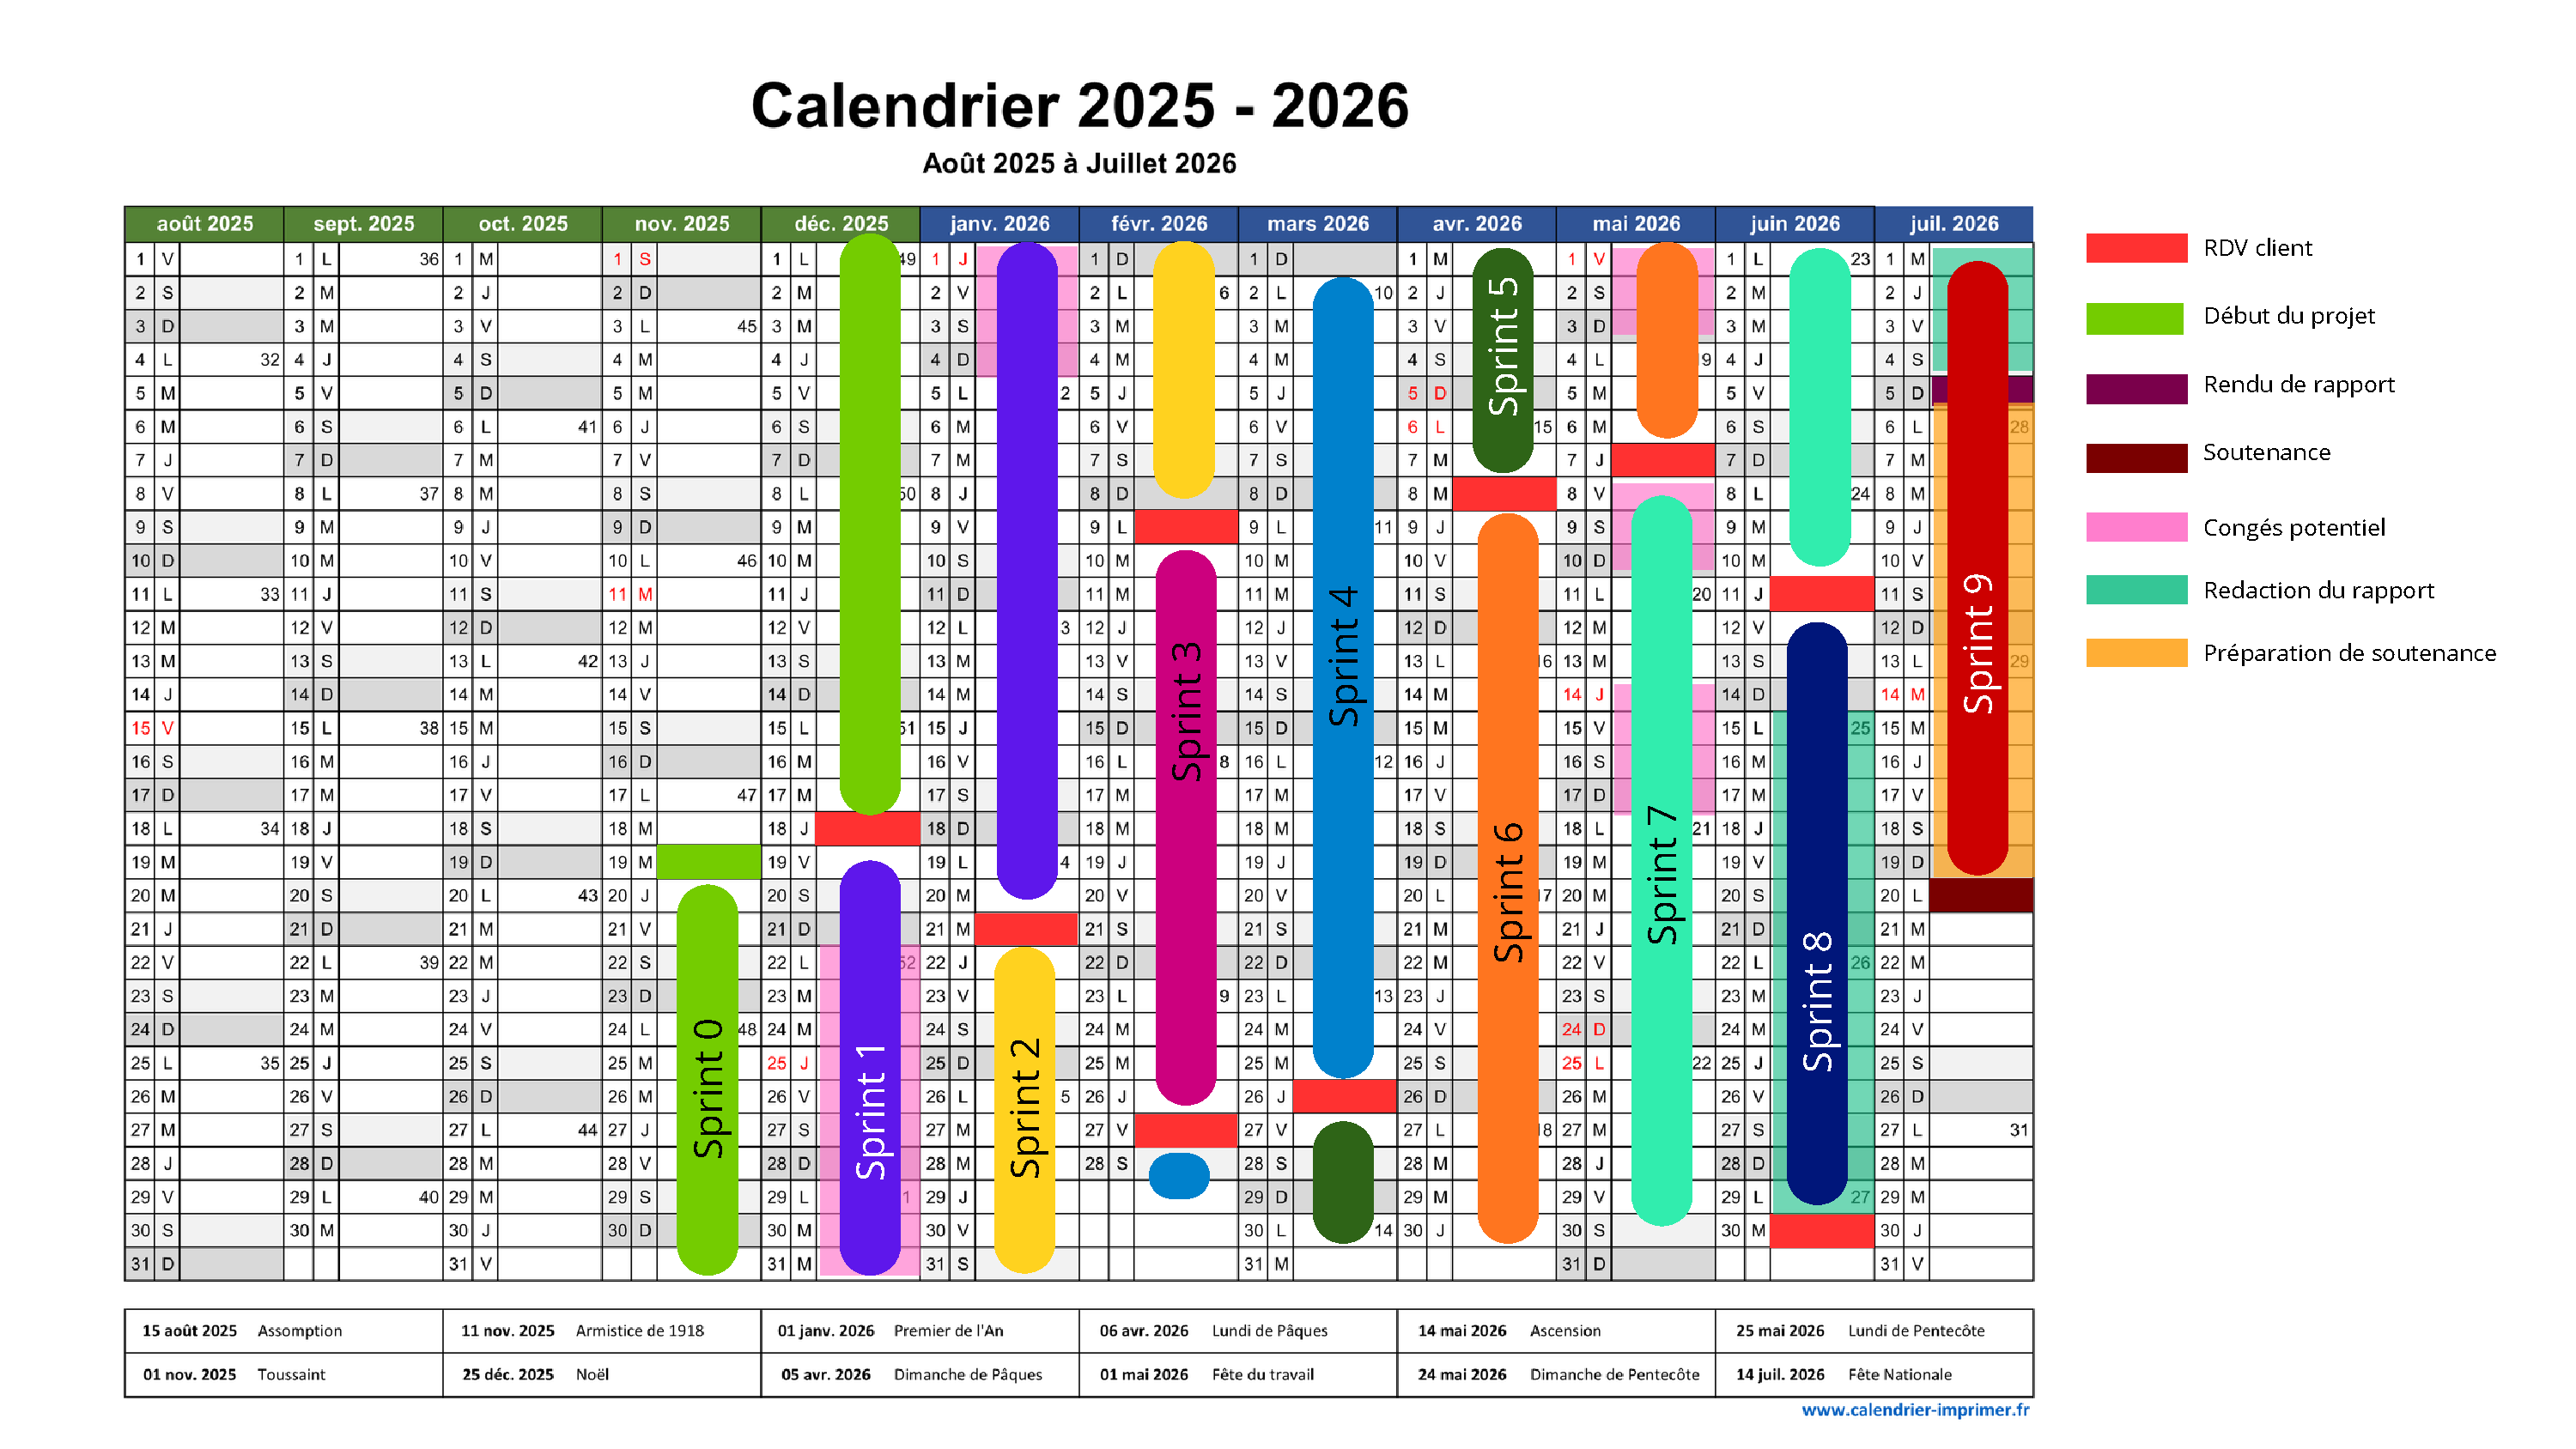
\includepdf[
  pages=-,
  pagecommand={\thispagestyle{plain}}
]{figures/annexes/ipf/calendrier_directeur.pdf}

\chapter{Diagramme de Gantt complet du projet Lynx Immo}
\label{ann:ipf-gantt-complet}

Le diagramme suivant restitue le planning détaillé du projet. Il permet d'examiner les dépendances, les périodes de réalisation et l'enchaînement des travaux qui ne peuvent être représentés intégralement dans le corps du dossier.

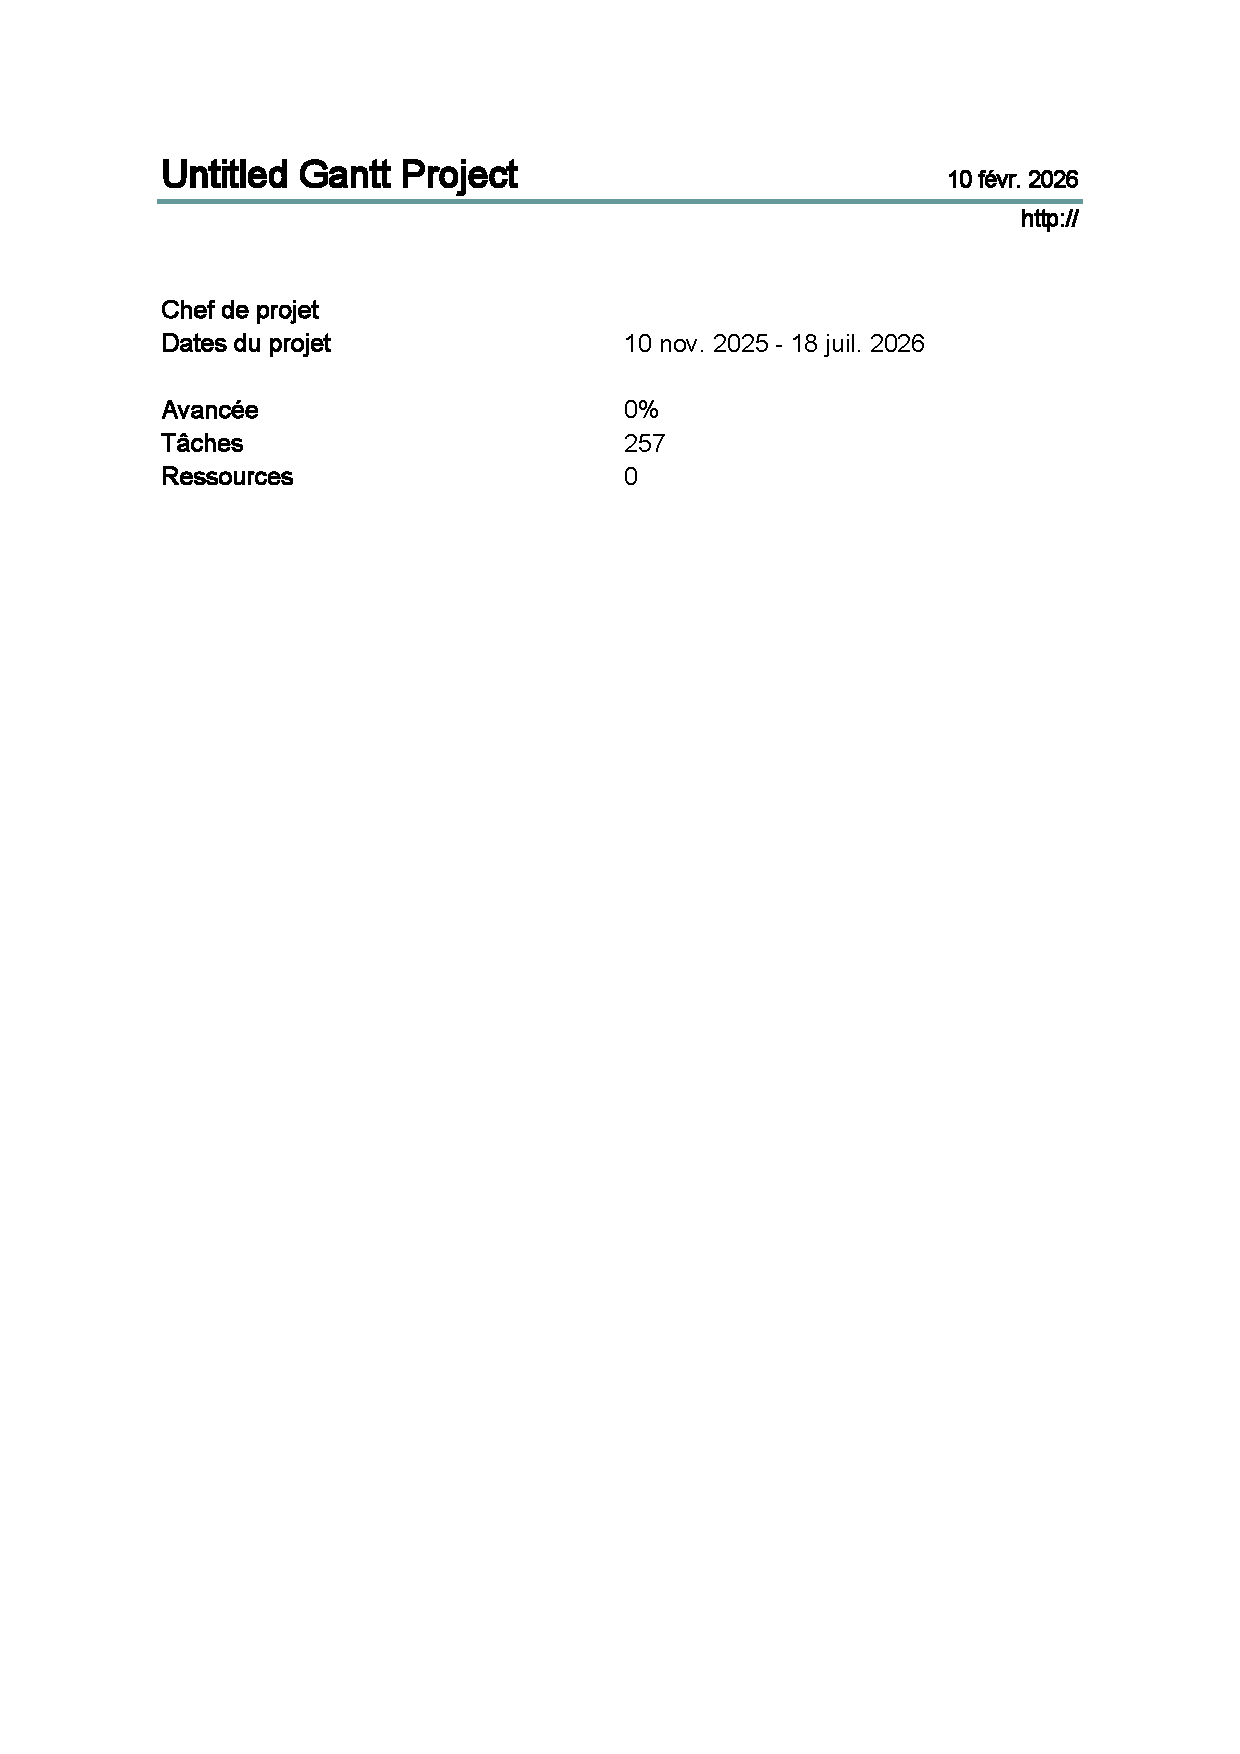
\includepdf[
  pages=-,
  pagecommand={\thispagestyle{plain}}
]{figures/annexes/ipf/gant_complet.pdf}

\chapter{Matrice de synthèse des exigences}
\label{ann:ipf-matrice-exigences}

Cette matrice fournit une vue consolidée de l'état des exigences et complète les tableaux détaillés reproduits dans les annexes suivantes.

\begin{figure}[H]
  \centering
  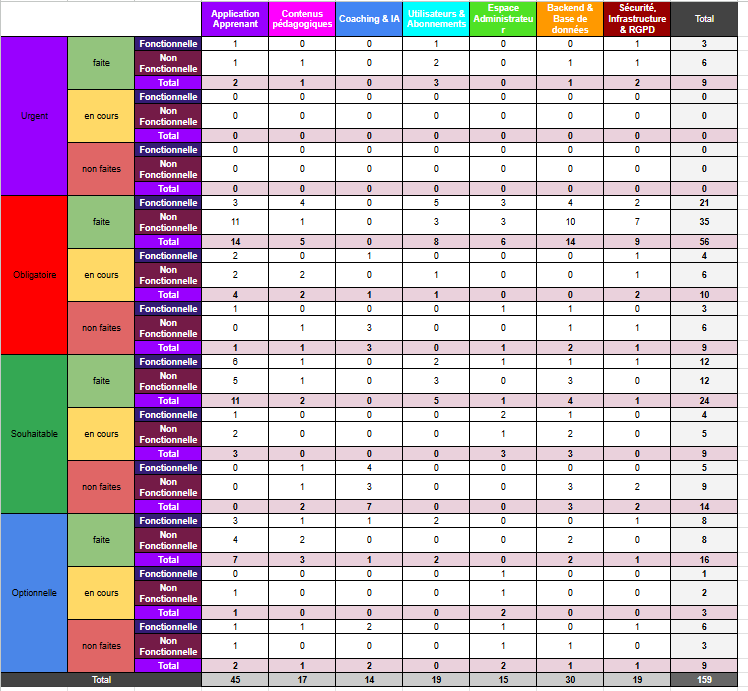
\includegraphics[width=\textwidth,height=0.78\textheight,keepaspectratio]{figures/annexes/ipf/matrice_synthese_exigences.png}
  \caption{Matrice de synthèse des exigences du projet Lynx Immo}
\end{figure}

\chapter{Personae et parcours utilisateurs}\label{annexe:persona}



\subsection{Présentation des personae}

Les personae représentent des profils types d’utilisateurs du projet \emph{5 Secondes Chrono}.
Ils permettent d’orienter les choix fonctionnels, l’ergonomie et les priorités du produit
en s’appuyant sur des besoins réalistes.

Chaque persona comprend :
\begin{itemize}
    \item un nom (fictif) et une tranche d’âge ;
    \item un contexte d’utilisation ;
    \item des motivations et objectifs ;
    \item des frustrations (points de douleur) ;
    \item une citation synthétisant son état d’esprit.
\end{itemize}

\subsection{Personae retenus pour \emph{5 Secondes Chrono}}

\begin{table}[h!]
\centering
\renewcommand{\arraystretch}{1.2}
\small
\begin{tabular}{|p{2.6cm}|p{3.2cm}|p{4.9cm}|p{4.9cm}|}
\hline
\rowcolor{etnaBlue!15}
\textbf{Persona} & \textbf{Profil / Contexte} & \textbf{Motivations / Objectifs} & \textbf{Frustrations} \\ \hline

\textbf{Nicolas (32 ans)} &
Négociateur en immobilier commercial. Utilise l’app le matin ou entre deux RDV. &
Monter en compétences rapidement ; réviser des notions clés ; progresser sans y passer 1h. &
Manque de temps ; contenus trop denses ; outils non adaptés au mobile ; peur de ``perdre son niveau''. \\ \hline

\textbf{Sarah (27 ans)} &
Jeune professionnelle en prise de poste. Utilise l’app le soir en micro-sessions. &
Se sentir à l’aise sur les bases juridiques ; apprendre de manière structurée ; avoir un feedback motivant. &
Stress d’erreur ; manque d’accompagnement ; difficulté à savoir quoi réviser ; besoin d’encouragements. \\ \hline

\textbf{Karim (41 ans)} &
Indépendant, agenda chargé. Utilise l’app de façon irrégulière. &
Réviser ponctuellement ; accéder rapidement à une explication (vidéo) ; gagner en confiance. &
Oublie de revenir ; n’aime pas les interfaces complexes ; abandon si la valeur n’est pas immédiate. \\ \hline

\textbf{Claire (35 ans)} &
Administratrice / formateur côté \emph{Le Carré Pro}. Gère contenus et suivi. &
Ajouter/mettre à jour les questions/vidéos ; suivre la progression ; s’assurer de la qualité pédagogique. &
Processus de gestion fastidieux ; manque de visibilité sur l’engagement ; crainte d’erreurs de contenu. \\ \hline

\end{tabular}
\caption{Personae principaux du projet \emph{5 Secondes Chrono}}
\end{table}

\subsection{Parcours utilisateurs}

Les parcours utilisateurs décrivent les étapes suivies par un persona pour atteindre un objectif.
Ils permettent d’identifier les points de friction, les besoins d’assistance et les priorités
d’interface.

Le projet \emph{5 Secondes Chrono} suit un parcours apprenant type :
\emph{Accueil $\rightarrow$ Quiz du jour $\rightarrow$ Résultats $\rightarrow$ Progression $\rightarrow$ Recommandations}.
Ce flux correspond au parcours macro défini pour l’application. \par
\noindent\textit{(Référence : séquence fonctionnelle globale du projet)} \textbf{---} \emph{Accueil / Quiz / Résultats / Progression / Reco}. \hfill

\subsection{Parcours utilisateur 1 — Réaliser le quiz quotidien (Nicolas)}

\begin{table}[h!]
\centering
\renewcommand{\arraystretch}{1.15}
\small
\begin{tabular}{|p{3.2cm}|p{10.4cm}|}
\hline
\rowcolor{black!10}
\textbf{Étape} & \textbf{Action / Résultat attendu} \\ \hline
Point d’entrée & Nicolas ouvre l’application depuis son téléphone (session courte). \\ \hline
Quiz du jour & Il lance le quiz quotidien et répond aux questions avec le timer. \\ \hline
Résultats & Il consulte son score et les explications associées (dont vidéo si disponible). \\ \hline
Progression & Il visualise son niveau / sa progression (thèmes maîtrisés vs à revoir). \\ \hline
Recommandations & Il reçoit une recommandation simple (notion à revoir / contenu conseillé). \\ \hline
Fin & Il quitte l’application en ayant le sentiment d’avoir progressé en moins de 2 minutes. \\ \hline
\end{tabular}
\caption{Parcours utilisateur — Quiz quotidien}
\end{table}

\subsection{Parcours utilisateur 2 — Se remettre à niveau grâce aux recommandations (Sarah)}

\begin{table}[h!]
\centering
\renewcommand{\arraystretch}{1.15}
\small
\begin{tabular}{|p{3.2cm}|p{10.4cm}|}
\hline
\rowcolor{black!10}
\textbf{Étape} & \textbf{Action / Résultat attendu} \\ \hline
Point d’entrée & Sarah ouvre l’app après une journée de travail, objectif : réviser ``utile''. \\ \hline
Progression & Elle consulte ses statistiques et repère une thématique en difficulté. \\ \hline
Recommandations & L’app suggère un quiz ciblé / une vidéo liée à ses erreurs fréquentes. \\ \hline
Contenu & Elle regarde une vidéo courte ou lit une explication avant de relancer un quiz. \\ \hline
Résultats & Elle vérifie l’amélioration de son score sur le thème concerné. \\ \hline
Fin & Elle ressort rassurée, avec une action claire pour la prochaine session. \\ \hline
\end{tabular}
\caption{Parcours utilisateur — Remédiation par recommandations}
\end{table}

\subsection{Parcours utilisateur 3 — Usage irrégulier mais efficace (Karim)}

\begin{table}[h!]
\centering
\renewcommand{\arraystretch}{1.15}
\small
\begin{tabular}{|p{3.2cm}|p{10.4cm}|}
\hline
\rowcolor{black!10}
\textbf{Étape} & \textbf{Action / Résultat attendu} \\ \hline
Point d’entrée & Karim relance l’app après plusieurs jours sans usage. \\ \hline
Accueil & L’app propose un accès direct au quiz et un rappel rapide de sa progression. \\ \hline
Quiz du jour & Il réalise une session courte, sans configuration complexe. \\ \hline
Résultats & Il comprend immédiatement ce qu’il a raté et pourquoi (explication claire). \\ \hline
Fin & Il obtient une valeur immédiate et est incité à revenir (gamification légère). \\ \hline
\end{tabular}
\caption{Parcours utilisateur — Reprise rapide}
\end{table}

\subsection{Parcours utilisateur 4 — Gestion des contenus (Claire, administratrice)}

\begin{table}[h!]
\centering
\renewcommand{\arraystretch}{1.15}
\small
\begin{tabular}{|p{3.2cm}|p{10.4cm}|}
\hline
\rowcolor{black!10}
\textbf{Étape} & \textbf{Action / Résultat attendu} \\ \hline
Point d’entrée & Claire se connecte à l’espace administrateur (web). \\ \hline
Gestion contenus & Elle ajoute/édite une question et associe une vidéo à une thématique. \\ \hline
Contrôle qualité & Elle vérifie la cohérence et la formulation (validation interne). \\ \hline
Publication & Les contenus deviennent disponibles selon les règles d’accès (abonnement). \\ \hline
Suivi & Elle consulte des statistiques (engagement, difficultés fréquentes). \\ \hline
Fin & Elle ajuste le contenu pédagogique selon les retours et les données observées. \\ \hline
\end{tabular}
\caption{Parcours utilisateur — Administration des contenus}
\end{table}



\chapter{Exigences fonctionnelles détaillées}
\label{ann:ipf-exigences-fonctionnelles}

Le tableau suivant reprend l'ensemble des exigences fonctionnelles, leur secteur, leur niveau de priorité et leur état en fin de projet.


\begingroup
\scriptsize
\setlength{\tabcolsep}{3pt}
\renewcommand{\arraystretch}{1.28}
\begin{longtable}{|P{1.75cm}|P{2.65cm}|P{7.45cm}|P{1.80cm}|P{1.55cm}|}
\caption{Exigences fonctionnelles}\\
\hline
\rowcolor{reqHeader}
\textcolor{white}{\textbf{N° référence}} & \textcolor{white}{\textbf{Secteur}} & \textcolor{white}{\textbf{Description}} & \textcolor{white}{\textbf{Importance}} & \textcolor{white}{\textbf{Fait/non fait}} \\ \hline
\endfirsthead
\hline
\rowcolor{reqHeader}
\textcolor{white}{\textbf{N° référence}} & \textcolor{white}{\textbf{Secteur}} & \textcolor{white}{\textbf{Description}} & \textcolor{white}{\textbf{Importance}} & \textcolor{white}{\textbf{Fait/non fait}} \\ \hline
\endhead
EF-S1-01 & \cellcolor{sectorColor0}\textcolor{white}{\textbf{Application Apprenant}} & L’utilisateur doit pouvoir lancer un quiz quotidien depuis l’écran principal. Le quiz contient une question aléatoire adaptée à son niveau ou thème sélectionné. & \reqtag{reqObligatoire}{white}{Obligatoire} & \reqtag{statusFait}{white}{Fait} \\ \hline
EF-S1-02 & \cellcolor{sectorColor0}\textcolor{white}{\textbf{Application Apprenant}} & L’application doit afficher une question QCM avec un timer fixe ou variable (selon décision client). À expiration, la réponse est considérée comme incorrecte. & \reqtag{reqUrgent}{white}{Urgent} & \reqtag{statusFait}{white}{Fait} \\ \hline
EF-S1-03 & \cellcolor{sectorColor0}\textcolor{white}{\textbf{Application Apprenant}} & L’utilisateur peut sélectionner un type de bail (Commercial, Professionnel, Dérogatoire…) avant de lancer un quiz. & \reqtag{reqObligatoire}{white}{Obligatoire} & \reqtag{statusFait}{white}{Fait} \\ \hline
EF-S1-04 & \cellcolor{sectorColor0}\textcolor{white}{\textbf{Application Apprenant}} & L’application doit afficher immédiatement si la réponse est correcte, avec un petit message ou une animation. & \reqtag{reqObligatoire}{white}{Obligatoire} & \reqtag{statusFait}{white}{Fait} \\ \hline
EF-S1-05 & \cellcolor{sectorColor0}\textcolor{white}{\textbf{Application Apprenant}} & Après la réponse, l’utilisateur doit pouvoir visionner la vidéo liée à la question. & \reqtag{reqObligatoire}{white}{Obligatoire} & \reqtag{statusEnCours}{black}{En cours} \\ \hline
EF-S1-06 & \cellcolor{sectorColor0}\textcolor{white}{\textbf{Application Apprenant}} & Chaque quiz attribue des points selon la vitesse et l’exactitude de la réponse. & \reqtag{reqSouhaitable}{white}{Souhaitable} & \reqtag{statusFait}{white}{Fait} \\ \hline
EF-S1-07 & \cellcolor{sectorColor0}\textcolor{white}{\textbf{Application Apprenant}} & L’application doit afficher l’évolution des scores, niveaux, erreurs fréquentes et progression par thématique. & \reqtag{reqObligatoire}{white}{Obligatoire} & \reqtag{statusEnCours}{black}{En cours} \\ \hline
EF-S1-08 & \cellcolor{sectorColor0}\textcolor{white}{\textbf{Application Apprenant}} & L’utilisateur reçoit une notification pour rappeler son quiz du jour. & \reqtag{reqOptionnelle}{white}{Optionnelle} & \reqtag{statusNonFait}{white}{Non fait} \\ \hline
EF-S1-09 & \cellcolor{sectorColor0}\textcolor{white}{\textbf{Application Apprenant}} & L’utilisateur doit pouvoir consulter ses questions passées, ses erreurs et les explications. & \reqtag{reqSouhaitable}{white}{Souhaitable} & \reqtag{statusFait}{white}{Fait} \\ \hline
EF-S1-10 & \cellcolor{sectorColor0}\textcolor{white}{\textbf{Application Apprenant}} & L’utilisateur peut sélectionner une thématique spécifique pour s’entraîner (ex : clauses du bail, fiscalité…). & \reqtag{reqSouhaitable}{white}{Souhaitable} & \reqtag{statusFait}{white}{Fait} \\ \hline
EF-S1-11 & \cellcolor{sectorColor0}\textcolor{white}{\textbf{Application Apprenant}} & L’utilisateur peut passer la vidéo explicative après une question. & \reqtag{reqSouhaitable}{white}{Souhaitable} & \reqtag{statusEnCours}{black}{En cours} \\ \hline
EF-S1-12 & \cellcolor{sectorColor0}\textcolor{white}{\textbf{Application Apprenant}} & L’application doit permettre à l’utilisateur de revoir les vidéos consultées dans son historique. & \reqtag{reqObligatoire}{white}{Obligatoire} & \reqtag{statusNonFait}{white}{Non fait} \\ \hline
EF-S1-13 & \cellcolor{sectorColor0}\textcolor{white}{\textbf{Application Apprenant}} & Lorsqu’un utilisateur fait trop d’erreurs sur une thématique, l’application propose automatiquement une session de révision ciblée. & \reqtag{reqSouhaitable}{white}{Souhaitable} & \reqtag{statusFait}{white}{Fait} \\ \hline
EF-S1-14 & \cellcolor{sectorColor0}\textcolor{white}{\textbf{Application Apprenant}} & L’utilisateur débloque des badges lors de jalons (10 quiz réussis, 3 jours consécutifs…). & \reqtag{reqOptionnelle}{white}{Optionnelle} & \reqtag{statusFait}{white}{Fait} \\ \hline
EF-S1-15 & \cellcolor{sectorColor0}\textcolor{white}{\textbf{Application Apprenant}} & L’utilisateur voit son niveau actuel et le nombre de points requis pour atteindre le niveau suivant. & \reqtag{reqSouhaitable}{white}{Souhaitable} & \reqtag{statusFait}{white}{Fait} \\ \hline
EF-S1-16 & \cellcolor{sectorColor0}\textcolor{white}{\textbf{Application Apprenant}} & Une animation visuelle doit signaler le décompte de 5 secondes (barre, cercle, couleur). & \reqtag{reqSouhaitable}{white}{Souhaitable} & \reqtag{statusFait}{white}{Fait} \\ \hline
EF-S1-17 & \cellcolor{sectorColor0}\textcolor{white}{\textbf{Application Apprenant}} & L’utilisateur peut sélectionner un thème sombre pour améliorer l’ergonomie en basse luminosité. & \reqtag{reqOptionnelle}{white}{Optionnelle} & \reqtag{statusFait}{white}{Fait} \\ \hline
EF-S1-18 & \cellcolor{sectorColor0}\textcolor{white}{\textbf{Application Apprenant}} & L’utilisateur peut enchaîner plusieurs quiz s’il le souhaite (selon sa formule). & \reqtag{reqOptionnelle}{white}{Optionnelle} & \reqtag{statusFait}{white}{Fait} \\ \hline
EF-S2-01 & \cellcolor{sectorColor1}\textcolor{white}{\textbf{Contenus pédagogiques}} & Le système doit stocker toutes les questions avec leurs réponses, explication et thématique. & \reqtag{reqObligatoire}{white}{Obligatoire} & \reqtag{statusFait}{white}{Fait} \\ \hline
EF-S2-02 & \cellcolor{sectorColor1}\textcolor{white}{\textbf{Contenus pédagogiques}} & Chaque question doit appartenir à une thématique juridique (ex : fonds de commerce). & \reqtag{reqObligatoire}{white}{Obligatoire} & \reqtag{statusFait}{white}{Fait} \\ \hline
EF-S2-03 & \cellcolor{sectorColor1}\textcolor{white}{\textbf{Contenus pédagogiques}} & Une vidéo explicative doit être liée à une ou plusieurs questions correspondantes. & \reqtag{reqObligatoire}{white}{Obligatoire} & \reqtag{statusFait}{white}{Fait} \\ \hline
EF-S2-04 & \cellcolor{sectorColor1}\textcolor{white}{\textbf{Contenus pédagogiques}} & Le système doit permettre d’ajouter, modifier ou supprimer des vidéos. & \reqtag{reqObligatoire}{white}{Obligatoire} & \reqtag{statusFait}{white}{Fait} \\ \hline
EF-S2-05 & \cellcolor{sectorColor1}\textcolor{white}{\textbf{Contenus pédagogiques}} & Chaque question possède un niveau (débutant, intermédiaire, expert). Le système choisit la difficulté en fonction du niveau utilisateur. & \reqtag{reqSouhaitable}{white}{Souhaitable} & \reqtag{statusFait}{white}{Fait} \\ \hline
EF-S2-06 & \cellcolor{sectorColor1}\textcolor{white}{\textbf{Contenus pédagogiques}} & Le modèle doit autoriser des questions avec plusieurs bonnes réponses pour les futures évolutions. & \reqtag{reqOptionnelle}{white}{Optionnelle} & \reqtag{statusNonFait}{white}{Non fait} \\ \hline
EF-S2-07 & \cellcolor{sectorColor1}\textcolor{white}{\textbf{Contenus pédagogiques}} & Les contenus ajoutés par les admins nécessitent une validation par Le Carré Pro avant publication. & \reqtag{reqSouhaitable}{white}{Souhaitable} & \reqtag{statusNonFait}{white}{Non fait} \\ \hline
EF-S2-08 & \cellcolor{sectorColor1}\textcolor{white}{\textbf{Contenus pédagogiques}} & Chaque question peut inclure une référence légale (article de loi, jurisprudence). & \reqtag{reqOptionnelle}{white}{Optionnelle} & \reqtag{statusFait}{white}{Fait} \\ \hline
EF-S3-01 & \cellcolor{sectorColor2}\textcolor{white}{\textbf{Coaching \& IA}} & Le système doit analyser les erreurs fréquentes et la rapidité de réponse. & \reqtag{reqObligatoire}{white}{Obligatoire} & \reqtag{statusEnCours}{black}{En cours} \\ \hline
EF-S3-02 & \cellcolor{sectorColor2}\textcolor{white}{\textbf{Coaching \& IA}} & L’application propose automatiquement une vidéo pertinente en cas de difficulté sur un thème. & \reqtag{reqSouhaitable}{white}{Souhaitable} & \reqtag{statusNonFait}{white}{Non fait} \\ \hline
EF-S3-03 & \cellcolor{sectorColor2}\textcolor{white}{\textbf{Coaching \& IA}} & L’application envoie des messages adaptés au profil (motivation, conseils, remédiation). & \reqtag{reqSouhaitable}{white}{Souhaitable} & \reqtag{statusNonFait}{white}{Non fait} \\ \hline
EF-S3-04 & \cellcolor{sectorColor2}\textcolor{white}{\textbf{Coaching \& IA}} & Le système doit maintenir un profil dynamique simple (ex : rapide mais imprécis). & \reqtag{reqOptionnelle}{white}{Optionnelle} & \reqtag{statusNonFait}{white}{Non fait} \\ \hline
EF-S3-05 & \cellcolor{sectorColor2}\textcolor{white}{\textbf{Coaching \& IA}} & Le système calcule un score d’apprentissage basé sur les réponses correctes/incorrectes et la vitesse. & \reqtag{reqSouhaitable}{white}{Souhaitable} & \reqtag{statusNonFait}{white}{Non fait} \\ \hline
EF-S3-06 & \cellcolor{sectorColor2}\textcolor{white}{\textbf{Coaching \& IA}} & L’IA détecte une baisse d’activité (ex : aucune réponse 3 jours) et déclenche un message motivant. & \reqtag{reqOptionnelle}{white}{Optionnelle} & \reqtag{statusNonFait}{white}{Non fait} \\ \hline
EF-S3-07 & \cellcolor{sectorColor2}\textcolor{white}{\textbf{Coaching \& IA}} & L’application propose un petit plan individuel de révision basé sur les erreurs fréquentes. & \reqtag{reqOptionnelle}{white}{Optionnelle} & \reqtag{statusFait}{white}{Fait} \\ \hline
EF-S3-08 & \cellcolor{sectorColor2}\textcolor{white}{\textbf{Coaching \& IA}} & L’application propose des conseils pratiques (ex : \og{}Revois les baux dérogatoires, où tu rates 40\% des questions\fg{}). & \reqtag{reqSouhaitable}{white}{Souhaitable} & \reqtag{statusNonFait}{white}{Non fait} \\ \hline
EF-S4-01 & \cellcolor{sectorColor3}\textcolor{white}{\textbf{Utilisateurs \& Abonnements}} & L’utilisateur peut créer un compte avec email et mot de passe. & \reqtag{reqObligatoire}{white}{Obligatoire} & \reqtag{statusFait}{white}{Fait} \\ \hline
EF-S4-02 & \cellcolor{sectorColor3}\textcolor{white}{\textbf{Utilisateurs \& Abonnements}} & Authentification sécurisée via JWT ou OAuth2. & \reqtag{reqUrgent}{white}{Urgent} & \reqtag{statusFait}{white}{Fait} \\ \hline
EF-S4-03 & \cellcolor{sectorColor3}\textcolor{white}{\textbf{Utilisateurs \& Abonnements}} & Le système détermine automatiquement les accès selon la formule souscrite. & \reqtag{reqObligatoire}{white}{Obligatoire} & \reqtag{statusFait}{white}{Fait} \\ \hline
EF-S4-04 & \cellcolor{sectorColor3}\textcolor{white}{\textbf{Utilisateurs \& Abonnements}} & L’utilisateur peut souscrire une formule via un système de paiement en ligne. & \reqtag{reqSouhaitable}{white}{Souhaitable} & \reqtag{statusFait}{white}{Fait} \\ \hline
EF-S4-05 & \cellcolor{sectorColor3}\textcolor{white}{\textbf{Utilisateurs \& Abonnements}} & Le système doit contrôler que chaque utilisateur a les droits correspondant à son abonnement. & \reqtag{reqObligatoire}{white}{Obligatoire} & \reqtag{statusFait}{white}{Fait} \\ \hline
EF-S4-06 & \cellcolor{sectorColor3}\textcolor{white}{\textbf{Utilisateurs \& Abonnements}} & Dès la connexion, l’application dirige l’utilisateur vers les écrans correspondant à son type d’abonnement. & \reqtag{reqObligatoire}{white}{Obligatoire} & \reqtag{statusFait}{white}{Fait} \\ \hline
EF-S4-07 & \cellcolor{sectorColor3}\textcolor{white}{\textbf{Utilisateurs \& Abonnements}} & L’utilisateur peut à tout moment passer d’Apprenti \ensuremath{\rightarrow} Compagnon \ensuremath{\rightarrow} Réussite. & \reqtag{reqSouhaitable}{white}{Souhaitable} & \reqtag{statusFait}{white}{Fait} \\ \hline
EF-S4-08 & \cellcolor{sectorColor3}\textcolor{white}{\textbf{Utilisateurs \& Abonnements}} & L’utilisateur peut suspendre temporairement son abonnement (fonction à valider avec Le Carré Pro). & \reqtag{reqOptionnelle}{white}{Optionnelle} & \reqtag{statusFait}{white}{Fait} \\ \hline
EF-S4-09 & \cellcolor{sectorColor3}\textcolor{white}{\textbf{Utilisateurs \& Abonnements}} & Le visiteur peut tester 1 quiz gratuit mais n’accède pas aux vidéos ni au coaching. & \reqtag{reqObligatoire}{white}{Obligatoire} & \reqtag{statusFait}{white}{Fait} \\ \hline
EF-S4-10 & \cellcolor{sectorColor3}\textcolor{white}{\textbf{Utilisateurs \& Abonnements}} & Le système doit être prêt à accueillir une authentification renforcée. & \reqtag{reqOptionnelle}{white}{Optionnelle} & \reqtag{statusFait}{white}{Fait} \\ \hline
EF-S5-01 & \cellcolor{sectorColor4}\textcolor{white}{\textbf{Tableau de bord Administrateur}} & L’administrateur peut ajouter, modifier, supprimer et visualiser les questions. & \reqtag{reqObligatoire}{white}{Obligatoire} & \reqtag{statusFait}{white}{Fait} \\ \hline
EF-S5-02 & \cellcolor{sectorColor4}\textcolor{white}{\textbf{Tableau de bord Administrateur}} & L’administrateur peut ajouter, lier, modifier et supprimer des vidéos. & \reqtag{reqObligatoire}{white}{Obligatoire} & \reqtag{statusFait}{white}{Fait} \\ \hline
EF-S5-03 & \cellcolor{sectorColor4}\textcolor{white}{\textbf{Tableau de bord Administrateur}} & L’administrateur doit avoir accès aux stats : abonnés, engagement, taux de réussite, revenus. & \reqtag{reqSouhaitable}{white}{Souhaitable} & \reqtag{statusEnCours}{black}{En cours} \\ \hline
EF-S5-04 & \cellcolor{sectorColor4}\textcolor{white}{\textbf{Tableau de bord Administrateur}} & L'administrateur peut visualiser et gérer les abonnements (activation, expiration). & \reqtag{reqObligatoire}{white}{Obligatoire} & \reqtag{statusNonFait}{white}{Non fait} \\ \hline
EF-S5-05 & \cellcolor{sectorColor4}\textcolor{white}{\textbf{Tableau de bord Administrateur}} & L’administrateur peut filtrer par type de bail, difficulté, date de création, validation. & \reqtag{reqSouhaitable}{white}{Souhaitable} & \reqtag{statusFait}{white}{Fait} \\ \hline
EF-S5-06 & \cellcolor{sectorColor4}\textcolor{white}{\textbf{Tableau de bord Administrateur}} & L’administrateur peut consulter la progression détaillée d’un abonné. & \reqtag{reqSouhaitable}{white}{Souhaitable} & \reqtag{statusEnCours}{black}{En cours} \\ \hline
EF-S5-07 & \cellcolor{sectorColor4}\textcolor{white}{\textbf{Tableau de bord Administrateur}} & L’administrateur peut exporter les résultats des quiz pour analyse externe. & \reqtag{reqOptionnelle}{white}{Optionnelle} & \reqtag{statusEnCours}{black}{En cours} \\ \hline
EF-S5-08 & \cellcolor{sectorColor4}\textcolor{white}{\textbf{Tableau de bord Administrateur}} & Le système doit permettre de définir plusieurs types d’admins (éditeur, superadmin). & \reqtag{reqOptionnelle}{white}{Optionnelle} & \reqtag{statusNonFait}{white}{Non fait} \\ \hline
EF-S5-09 & \cellcolor{sectorColor4}\textcolor{white}{\textbf{Tableau de bord Administrateur}} & L’admin peut prévisualiser une vidéo avant publication & \reqtag{reqObligatoire}{white}{Obligatoire} & \reqtag{statusFait}{white}{Fait} \\ \hline
EF-S6-01 & \cellcolor{sectorColor5}\textcolor{white}{\textbf{Backend / API \& Base de Données}} & L’API doit fournir une question aléatoire selon le niveau et le type de bail. & \reqtag{reqObligatoire}{white}{Obligatoire} & \reqtag{statusFait}{white}{Fait} \\ \hline
EF-S6-02 & \cellcolor{sectorColor5}\textcolor{white}{\textbf{Backend / API \& Base de Données}} & L’API doit renvoyer la vidéo associée à une question. & \reqtag{reqObligatoire}{white}{Obligatoire} & \reqtag{statusFait}{white}{Fait} \\ \hline
EF-S6-03 & \cellcolor{sectorColor5}\textcolor{white}{\textbf{Backend / API \& Base de Données}} & L’API doit permettre de récupérer et mettre à jour la progression d’un utilisateur. & \reqtag{reqObligatoire}{white}{Obligatoire} & \reqtag{statusFait}{white}{Fait} \\ \hline
EF-S6-04 & \cellcolor{sectorColor5}\textcolor{white}{\textbf{Backend / API \& Base de Données}} & L’API doit fournir une question aléatoire mais équilibrée selon la thématique et la difficulté. & \reqtag{reqSouhaitable}{white}{Souhaitable} & \reqtag{statusFait}{white}{Fait} \\ \hline
EF-S6-05 & \cellcolor{sectorColor5}\textcolor{white}{\textbf{Backend / API \& Base de Données}} & L’API doit retourner les thématiques majoritairement ratées par l’utilisateur. & \reqtag{reqObligatoire}{white}{Obligatoire} & \reqtag{statusNonFait}{white}{Non fait} \\ \hline
EF-S6-06 & \cellcolor{sectorColor5}\textcolor{white}{\textbf{Backend / API \& Base de Données}} & L’API fournit les données agrégées pour le tableau de bord admin. & \reqtag{reqObligatoire}{white}{Obligatoire} & \reqtag{statusFait}{white}{Fait} \\ \hline
EF-S6-07 & \cellcolor{sectorColor5}\textcolor{white}{\textbf{Backend / API \& Base de Données}} & L’API permet d’activer, suspendre, mettre à jour ou annuler un abonnement. & \reqtag{reqSouhaitable}{white}{Souhaitable} & \reqtag{statusEnCours}{black}{En cours} \\ \hline
EF-S7-01 & \cellcolor{sectorColor6}\textcolor{white}{\textbf{Sécurité, Infrastructure \& RGPD}} & Les données doivent être stockées de manière sécurisée, chiffrées au repos et en transit. & \reqtag{reqUrgent}{white}{Urgent} & \reqtag{statusFait}{white}{Fait} \\ \hline
EF-S7-02 & \cellcolor{sectorColor6}\textcolor{white}{\textbf{Sécurité, Infrastructure \& RGPD}} & L'utilisateur doit accepter les CGU et la politique RGPD. & \reqtag{reqObligatoire}{white}{Obligatoire} & \reqtag{statusEnCours}{black}{En cours} \\ \hline
EF-S7-03 & \cellcolor{sectorColor6}\textcolor{white}{\textbf{Sécurité, Infrastructure \& RGPD}} & Le système doit enregistrer les connexions et événements critiques. & \reqtag{reqOptionnelle}{white}{Optionnelle} & \reqtag{statusFait}{white}{Fait} \\ \hline
EF-S7-04 & \cellcolor{sectorColor6}\textcolor{white}{\textbf{Sécurité, Infrastructure \& RGPD}} & L’utilisateur doit pouvoir demander la suppression de son compte (RGPD). & \reqtag{reqObligatoire}{white}{Obligatoire} & \reqtag{statusFait}{white}{Fait} \\ \hline
EF-S7-05 & \cellcolor{sectorColor6}\textcolor{white}{\textbf{Sécurité, Infrastructure \& RGPD}} & Le système doit permettre à l’utilisateur d’obtenir ses données (CSV ou JSON). & \reqtag{reqOptionnelle}{white}{Optionnelle} & \reqtag{statusNonFait}{white}{Non fait} \\ \hline
EF-S7-06 & \cellcolor{sectorColor6}\textcolor{white}{\textbf{Sécurité, Infrastructure \& RGPD}} & L’application doit afficher les CGU, conditions d’abonnement et politique RGPD. & \reqtag{reqObligatoire}{white}{Obligatoire} & \reqtag{statusFait}{white}{Fait} \\ \hline
EF-S7-07 & \cellcolor{sectorColor6}\textcolor{white}{\textbf{Sécurité, Infrastructure \& RGPD}} & La base de données doit être sauvegardée quotidiennement. & \reqtag{reqSouhaitable}{white}{Souhaitable} & \reqtag{statusFait}{white}{Fait} \\ \hline
\end{longtable}
\endgroup


\chapter{Exigences non fonctionnelles détaillées}
\label{ann:ipf-exigences-non-fonctionnelles}

Le tableau suivant reprend les exigences non fonctionnelles relatives notamment à l'ergonomie, la performance, la sécurité, l'accessibilité, la maintenabilité, la documentation et la qualité de service.


\begingroup
\scriptsize
\setlength{\tabcolsep}{3pt}
\renewcommand{\arraystretch}{1.28}
\begin{longtable}{|P{2.15cm}|P{1.55cm}|P{2.35cm}|P{5.60cm}|P{1.65cm}|P{1.45cm}|}
\caption{Exigences non fonctionnelles}\\
\hline
\rowcolor{reqHeader}
\textcolor{white}{\textbf{Thématique}} & \textcolor{white}{\textbf{N° référence}} & \textcolor{white}{\textbf{Secteur}} & \textcolor{white}{\textbf{Description}} & \textcolor{white}{\textbf{Importance}} & \textcolor{white}{\textbf{Fait/non fait}} \\ \hline
\endfirsthead
\hline
\rowcolor{reqHeader}
\textcolor{white}{\textbf{Thématique}} & \textcolor{white}{\textbf{N° référence}} & \textcolor{white}{\textbf{Secteur}} & \textcolor{white}{\textbf{Description}} & \textcolor{white}{\textbf{Importance}} & \textcolor{white}{\textbf{Fait/non fait}} \\ \hline
\endhead
\rowcolor{themeColor0!18}
\cellcolor{themeColor0!45}\textcolor{black}{\textbf{GRAPHISME \& DESIGN}} & NF-G-01 & \cellcolor{sectorColor0}\textcolor{white}{\textbf{Application Apprenant}} & L’application doit respecter une charte graphique cohérente (couleurs, typographies, icônes). & \reqtag{reqObligatoire}{white}{Obligatoire} & \reqtag{statusFait}{white}{Fait} \\ \hline
\rowcolor{themeColor0!18}
\cellcolor{themeColor0!45}\textcolor{black}{\textbf{GRAPHISME \& DESIGN}} & NF-G-02 & \cellcolor{sectorColor0}\textcolor{white}{\textbf{Application Apprenant}} & Les écrans doivent s’adapter à toutes tailles d’écran mobile (petits et grands smartphones). & \reqtag{reqObligatoire}{white}{Obligatoire} & \reqtag{statusFait}{white}{Fait} \\ \hline
\rowcolor{themeColor0!18}
\cellcolor{themeColor0!45}\textcolor{black}{\textbf{GRAPHISME \& DESIGN}} & NF-G-03 & \cellcolor{sectorColor0}\textcolor{white}{\textbf{Application Apprenant}} & Les boutons, cartes, listes, modales et inputs doivent respecter un style stylisé et uniformisé. & \reqtag{reqSouhaitable}{white}{Souhaitable} & \reqtag{statusFait}{white}{Fait} \\ \hline
\rowcolor{themeColor0!18}
\cellcolor{themeColor0!45}\textcolor{black}{\textbf{GRAPHISME \& DESIGN}} & NF-G-04 & \cellcolor{sectorColor0}\textcolor{white}{\textbf{Application Apprenant}} & Les animations (timer, transitions, badges) doivent être légères, fluides et ne pas bloquer l’expérience. & \reqtag{reqOptionnelle}{white}{Optionnelle} & \reqtag{statusFait}{white}{Fait} \\ \hline
\rowcolor{themeColor1!18}
\cellcolor{themeColor1!45}\textcolor{black}{\textbf{ERGONOMIE \& UX}} & NF-UX-01 & \cellcolor{sectorColor0}\textcolor{white}{\textbf{Application Apprenant}} & L’utilisateur doit pouvoir lancer un quiz en maximum trois actions depuis l’accueil. & \reqtag{reqObligatoire}{white}{Obligatoire} & \reqtag{statusFait}{white}{Fait} \\ \hline
\rowcolor{themeColor1!18}
\cellcolor{themeColor1!45}\textcolor{black}{\textbf{ERGONOMIE \& UX}} & NF-UX-02 & \cellcolor{sectorColor0}\textcolor{white}{\textbf{Application Apprenant}} & Toute action utilisateur doit avoir un feedback immédiat (< 200 ms). & \reqtag{reqObligatoire}{white}{Obligatoire} & \reqtag{statusFait}{white}{Fait} \\ \hline
\rowcolor{themeColor1!18}
\cellcolor{themeColor1!45}\textcolor{black}{\textbf{ERGONOMIE \& UX}} & NF-UX-03 & \cellcolor{sectorColor0}\textcolor{white}{\textbf{Application Apprenant}} & Les parcours doivent être simples, lisibles et sans surcharge cognitive. & \reqtag{reqObligatoire}{white}{Obligatoire} & \reqtag{statusFait}{white}{Fait} \\ \hline
\rowcolor{themeColor1!18}
\cellcolor{themeColor1!45}\textcolor{black}{\textbf{ERGONOMIE \& UX}} & NF-UX-04 & \cellcolor{sectorColor0}\textcolor{white}{\textbf{Application Apprenant}} & Les contrastes doivent respecter les normes WCAG AA. & \reqtag{reqSouhaitable}{white}{Souhaitable} & \reqtag{statusEnCours}{black}{En cours} \\ \hline
\rowcolor{themeColor2!18}
\cellcolor{themeColor2!45}\textcolor{black}{\textbf{PERFORMANCE}} & NF-P-01 & \cellcolor{sectorColor1}\textcolor{white}{\textbf{Backend / API \& Base de Données}} & Temps de chargement des écrans < 1,5 seconde & \reqtag{reqUrgent}{white}{Urgent} & \reqtag{statusFait}{white}{Fait} \\ \hline
\rowcolor{themeColor2!18}
\cellcolor{themeColor2!45}\textcolor{black}{\textbf{PERFORMANCE}} & NF-P-02 & \cellcolor{sectorColor1}\textcolor{white}{\textbf{Backend / API \& Base de Données}} & Requête API quiz < 300 ms & \reqtag{reqObligatoire}{white}{Obligatoire} & \reqtag{statusFait}{white}{Fait} \\ \hline
\rowcolor{themeColor2!18}
\cellcolor{themeColor2!45}\textcolor{black}{\textbf{PERFORMANCE}} & NF-P-03 & \cellcolor{sectorColor2}\textcolor{white}{\textbf{Contenus pédagogiques}} & Optimisation des images \& vidéos & \reqtag{reqObligatoire}{white}{Obligatoire} & \reqtag{statusEnCours}{black}{En cours} \\ \hline
\rowcolor{themeColor2!18}
\cellcolor{themeColor2!45}\textcolor{black}{\textbf{PERFORMANCE}} & NF-P-04 & \cellcolor{sectorColor0}\textcolor{white}{\textbf{Application Apprenant}} & Application fluide même sur appareils modestes & \reqtag{reqSouhaitable}{white}{Souhaitable} & \reqtag{statusFait}{white}{Fait} \\ \hline
\rowcolor{themeColor2!18}
\cellcolor{themeColor2!45}\textcolor{black}{\textbf{PERFORMANCE}} & NF-P-05 & \cellcolor{sectorColor0}\textcolor{white}{\textbf{Application Apprenant}} & Temps de chargement des écrans < 1,5 seconde & \reqtag{reqUrgent}{white}{Urgent} & \reqtag{statusFait}{white}{Fait} \\ \hline
\rowcolor{themeColor2!18}
\cellcolor{themeColor2!45}\textcolor{black}{\textbf{PERFORMANCE}} & NF-P-06 & \cellcolor{sectorColor3}\textcolor{white}{\textbf{Tableau de bord Administrateur}} & Optimisation des images \& vidéos & \reqtag{reqObligatoire}{white}{Obligatoire} & \reqtag{statusFait}{white}{Fait} \\ \hline
\rowcolor{themeColor3!18}
\cellcolor{themeColor3!45}\textcolor{black}{\textbf{SÉCURITÉ \& AUTHENTIFICATION}} & NF-SEC-01 & \cellcolor{sectorColor4}\textcolor{white}{\textbf{Utilisateurs \& Abonnements}} & Authentification sécurisée JWT & \reqtag{reqUrgent}{white}{Urgent} & \reqtag{statusFait}{white}{Fait} \\ \hline
\rowcolor{themeColor3!18}
\cellcolor{themeColor3!45}\textcolor{black}{\textbf{SÉCURITÉ \& AUTHENTIFICATION}} & NF-SEC-02 & \cellcolor{sectorColor5}\textcolor{white}{\textbf{Sécurité, Infrastructure \& RGPD}} & Authentification sécurisée JWT & \reqtag{reqUrgent}{white}{Urgent} & \reqtag{statusFait}{white}{Fait} \\ \hline
\rowcolor{themeColor3!18}
\cellcolor{themeColor3!45}\textcolor{black}{\textbf{SÉCURITÉ \& AUTHENTIFICATION}} & NF-SEC-03 & \cellcolor{sectorColor5}\textcolor{white}{\textbf{Sécurité, Infrastructure \& RGPD}} & Stockage chiffré des mots de passe (hash + salt) & \reqtag{reqObligatoire}{white}{Obligatoire} & \reqtag{statusFait}{white}{Fait} \\ \hline
\rowcolor{themeColor3!18}
\cellcolor{themeColor3!45}\textcolor{black}{\textbf{SÉCURITÉ \& AUTHENTIFICATION}} & NF-SEC-04 & \cellcolor{sectorColor4}\textcolor{white}{\textbf{Utilisateurs \& Abonnements}} & Interdiction d’accès aux fonctionnalités restreintes sans abonnement valide & \reqtag{reqObligatoire}{white}{Obligatoire} & \reqtag{statusFait}{white}{Fait} \\ \hline
\rowcolor{themeColor3!18}
\cellcolor{themeColor3!45}\textcolor{black}{\textbf{SÉCURITÉ \& AUTHENTIFICATION}} & NF-SEC-05 & \cellcolor{sectorColor4}\textcolor{white}{\textbf{Utilisateurs \& Abonnements}} & Expiration automatique des sessions & \reqtag{reqObligatoire}{white}{Obligatoire} & \reqtag{statusFait}{white}{Fait} \\ \hline
\rowcolor{themeColor4!18}
\cellcolor{themeColor4!45}\textcolor{black}{\textbf{PROTECTION DES DONNÉES / RGPD}} & NF-RGPD-01 & \cellcolor{sectorColor5}\textcolor{white}{\textbf{Sécurité, Infrastructure \& RGPD}} & Consentement explicite & \reqtag{reqObligatoire}{white}{Obligatoire} & \reqtag{statusFait}{white}{Fait} \\ \hline
\rowcolor{themeColor4!18}
\cellcolor{themeColor4!45}\textcolor{black}{\textbf{PROTECTION DES DONNÉES / RGPD}} & NF-RGPD-02 & \cellcolor{sectorColor5}\textcolor{white}{\textbf{Sécurité, Infrastructure \& RGPD}} & Droit à l’oubli (suppression compte + données) & \reqtag{reqObligatoire}{white}{Obligatoire} & \reqtag{statusFait}{white}{Fait} \\ \hline
\rowcolor{themeColor4!18}
\cellcolor{themeColor4!45}\textcolor{black}{\textbf{PROTECTION DES DONNÉES / RGPD}} & NF-RGPD-03 & \cellcolor{sectorColor5}\textcolor{white}{\textbf{Sécurité, Infrastructure \& RGPD}} & Exportation des données personnelles & \reqtag{reqSouhaitable}{white}{Souhaitable} & \reqtag{statusNonFait}{white}{Non fait} \\ \hline
\rowcolor{themeColor4!18}
\cellcolor{themeColor4!45}\textcolor{black}{\textbf{PROTECTION DES DONNÉES / RGPD}} & NF-RGPD-04 & \cellcolor{sectorColor6}\textcolor{white}{\textbf{Coaching \& IA}} & Anonymisation des données pour l’IA & \reqtag{reqObligatoire}{white}{Obligatoire} & \reqtag{statusNonFait}{white}{Non fait} \\ \hline
\rowcolor{themeColor4!18}
\cellcolor{themeColor4!45}\textcolor{black}{\textbf{PROTECTION DES DONNÉES / RGPD}} & NF-RGPD-05 & \cellcolor{sectorColor5}\textcolor{white}{\textbf{Sécurité, Infrastructure \& RGPD}} & Anonymisation des données pour l’IA & \reqtag{reqObligatoire}{white}{Obligatoire} & \reqtag{statusNonFait}{white}{Non fait} \\ \hline
\rowcolor{themeColor5!18}
\cellcolor{themeColor5!45}\textcolor{black}{\textbf{FIABILITÉ \& DISPONIBILITÉ}} & NF-FD-01 & \cellcolor{sectorColor1}\textcolor{white}{\textbf{Backend / API \& Base de Données}} & Disponibilité cible : 99,5 \% & \reqtag{reqObligatoire}{white}{Obligatoire} & \reqtag{statusFait}{white}{Fait} \\ \hline
\rowcolor{themeColor5!18}
\cellcolor{themeColor5!45}\textcolor{black}{\textbf{FIABILITÉ \& DISPONIBILITÉ}} & NF-FD-02 & \cellcolor{sectorColor5}\textcolor{white}{\textbf{Sécurité, Infrastructure \& RGPD}} & Sauvegarde quotidienne de la base & \reqtag{reqObligatoire}{white}{Obligatoire} & \reqtag{statusFait}{white}{Fait} \\ \hline
\rowcolor{themeColor5!18}
\cellcolor{themeColor5!45}\textcolor{black}{\textbf{FIABILITÉ \& DISPONIBILITÉ}} & NF-FD-03 & \cellcolor{sectorColor1}\textcolor{white}{\textbf{Backend / API \& Base de Données}} & Tolérance aux erreurs API & \reqtag{reqSouhaitable}{white}{Souhaitable} & \reqtag{statusFait}{white}{Fait} \\ \hline
\rowcolor{themeColor5!18}
\cellcolor{themeColor5!45}\textcolor{black}{\textbf{FIABILITÉ \& DISPONIBILITÉ}} & NF-FD-04 & \cellcolor{sectorColor0}\textcolor{white}{\textbf{Application Apprenant}} & Message d’erreur clair et non technique & \reqtag{reqObligatoire}{white}{Obligatoire} & \reqtag{statusFait}{white}{Fait} \\ \hline
\rowcolor{themeColor5!18}
\cellcolor{themeColor5!45}\textcolor{black}{\textbf{FIABILITÉ \& DISPONIBILITÉ}} & NF-FD-05 & \cellcolor{sectorColor3}\textcolor{white}{\textbf{Tableau de bord Administrateur}} & Message d’erreur clair et non technique & \reqtag{reqObligatoire}{white}{Obligatoire} & \reqtag{statusFait}{white}{Fait} \\ \hline
\rowcolor{themeColor5!18}
\cellcolor{themeColor5!45}\textcolor{black}{\textbf{FIABILITÉ \& DISPONIBILITÉ}} & NF-FD-06 & \cellcolor{sectorColor5}\textcolor{white}{\textbf{Sécurité, Infrastructure \& RGPD}} & Disponibilité cible : 99,5 \% & \reqtag{reqObligatoire}{white}{Obligatoire} & \reqtag{statusFait}{white}{Fait} \\ \hline
\rowcolor{themeColor6!18}
\cellcolor{themeColor6!45}\textcolor{black}{\textbf{COMPATIBILITÉ \& ACCESSIBILITÉ}} & NF-COMP-01 & \cellcolor{sectorColor0}\textcolor{white}{\textbf{Application Apprenant}} & Compatibilité iOS et Android & \reqtag{reqObligatoire}{white}{Obligatoire} & \reqtag{statusFait}{white}{Fait} \\ \hline
\rowcolor{themeColor6!18}
\cellcolor{themeColor6!45}\textcolor{black}{\textbf{COMPATIBILITÉ \& ACCESSIBILITÉ}} & NF-COMP-02 & \cellcolor{sectorColor0}\textcolor{white}{\textbf{Application Apprenant}} & Fonctionnement sur Android 8+ et iOS 13+ & \reqtag{reqObligatoire}{white}{Obligatoire} & \reqtag{statusFait}{white}{Fait} \\ \hline
\rowcolor{themeColor6!18}
\cellcolor{themeColor6!45}\textcolor{black}{\textbf{COMPATIBILITÉ \& ACCESSIBILITÉ}} & NF-COMP-03 & \cellcolor{sectorColor0}\textcolor{white}{\textbf{Application Apprenant}} & Accessibilité boutons / contraste & \reqtag{reqSouhaitable}{white}{Souhaitable} & \reqtag{statusFait}{white}{Fait} \\ \hline
\rowcolor{themeColor6!18}
\cellcolor{themeColor6!45}\textcolor{black}{\textbf{COMPATIBILITÉ \& ACCESSIBILITÉ}} & NF-COMP-04 & \cellcolor{sectorColor0}\textcolor{white}{\textbf{Application Apprenant}} & Support des modes paysage / portrait & \reqtag{reqOptionnelle}{white}{Optionnelle} & \reqtag{statusNonFait}{white}{Non fait} \\ \hline
\rowcolor{themeColor7!18}
\cellcolor{themeColor7!45}\textcolor{black}{\textbf{MAINTENABILITÉ \& SCALABILITÉ}} & NF-MS-01 & \cellcolor{sectorColor1}\textcolor{white}{\textbf{Backend / API \& Base de Données}} & Code modulaire et documenté & \reqtag{reqObligatoire}{white}{Obligatoire} & \reqtag{statusFait}{white}{Fait} \\ \hline
\rowcolor{themeColor7!18}
\cellcolor{themeColor7!45}\textcolor{black}{\textbf{MAINTENABILITÉ \& SCALABILITÉ}} & NF-MS-02 & \cellcolor{sectorColor1}\textcolor{white}{\textbf{Backend / API \& Base de Données}} & Architecture API scalable & \reqtag{reqObligatoire}{white}{Obligatoire} & \reqtag{statusFait}{white}{Fait} \\ \hline
\rowcolor{themeColor7!18}
\cellcolor{themeColor7!45}\textcolor{black}{\textbf{MAINTENABILITÉ \& SCALABILITÉ}} & NF-MS-03 & \cellcolor{sectorColor1}\textcolor{white}{\textbf{Backend / API \& Base de Données}} & Logs structurés et exploitables & \reqtag{reqSouhaitable}{white}{Souhaitable} & \reqtag{statusEnCours}{black}{En cours} \\ \hline
\rowcolor{themeColor7!18}
\cellcolor{themeColor7!45}\textcolor{black}{\textbf{MAINTENABILITÉ \& SCALABILITÉ}} & NF-MS-04 & \cellcolor{sectorColor2}\textcolor{white}{\textbf{Contenus pédagogiques}} & Possibilité d’ajouter facilement de nouvelles thématiques de quiz & \reqtag{reqObligatoire}{white}{Obligatoire} & \reqtag{statusNonFait}{white}{Non fait} \\ \hline
\rowcolor{themeColor8!18}
\cellcolor{themeColor8!45}\textcolor{black}{\textbf{DOCUMENTATION \& TESTS}} & NF-DOC-01 & \cellcolor{sectorColor1}\textcolor{white}{\textbf{Backend / API \& Base de Données}} & Documentation API complète (Swagger) & \reqtag{reqObligatoire}{white}{Obligatoire} & \reqtag{statusFait}{white}{Fait} \\ \hline
\rowcolor{themeColor8!18}
\cellcolor{themeColor8!45}\textcolor{black}{\textbf{DOCUMENTATION \& TESTS}} & NF-DOC-02 & \cellcolor{sectorColor1}\textcolor{white}{\textbf{Backend / API \& Base de Données}} & Tests unitaires sur les modules critiques & \reqtag{reqObligatoire}{white}{Obligatoire} & \reqtag{statusNonFait}{white}{Non fait} \\ \hline
\rowcolor{themeColor8!18}
\cellcolor{themeColor8!45}\textcolor{black}{\textbf{DOCUMENTATION \& TESTS}} & NF-DOC-03 & \cellcolor{sectorColor0}\textcolor{white}{\textbf{Application Apprenant}} & Manuel utilisateur (apprenant + admin) & \reqtag{reqSouhaitable}{white}{Souhaitable} & \reqtag{statusEnCours}{black}{En cours} \\ \hline
\rowcolor{themeColor8!18}
\cellcolor{themeColor8!45}\textcolor{black}{\textbf{DOCUMENTATION \& TESTS}} & NF-DOC-04 & \cellcolor{sectorColor3}\textcolor{white}{\textbf{Tableau de bord Administrateur}} & Manuel utilisateur (apprenant + admin) & \reqtag{reqSouhaitable}{white}{Souhaitable} & \reqtag{statusEnCours}{black}{En cours} \\ \hline
\rowcolor{themeColor8!18}
\cellcolor{themeColor8!45}\textcolor{black}{\textbf{DOCUMENTATION \& TESTS}} & NF-DOC-05 & \cellcolor{sectorColor1}\textcolor{white}{\textbf{Backend / API \& Base de Données}} & Historique des versions (changelog) & \reqtag{reqOptionnelle}{white}{Optionnelle} & \reqtag{statusNonFait}{white}{Non fait} \\ \hline
\rowcolor{themeColor9!18}
\cellcolor{themeColor9!45}\textcolor{black}{\textbf{CONFORMITÉ LÉGALE}} & NF-LEG-01 & \cellcolor{sectorColor4}\textcolor{white}{\textbf{Utilisateurs \& Abonnements}} & CGU obligatoires à accepter & \reqtag{reqObligatoire}{white}{Obligatoire} & \reqtag{statusFait}{white}{Fait} \\ \hline
\rowcolor{themeColor9!18}
\cellcolor{themeColor9!45}\textcolor{black}{\textbf{CONFORMITÉ LÉGALE}} & NF-LEG-02 & \cellcolor{sectorColor0}\textcolor{white}{\textbf{Application Apprenant}} & Mentions légales accessibles & \reqtag{reqObligatoire}{white}{Obligatoire} & \reqtag{statusEnCours}{black}{En cours} \\ \hline
\rowcolor{themeColor9!18}
\cellcolor{themeColor9!45}\textcolor{black}{\textbf{CONFORMITÉ LÉGALE}} & NF-LEG-03 & \cellcolor{sectorColor2}\textcolor{white}{\textbf{Contenus pédagogiques}} & Respect des droits d’auteur pour les vidéos & \reqtag{reqObligatoire}{white}{Obligatoire} & \reqtag{statusFait}{white}{Fait} \\ \hline
\rowcolor{themeColor9!18}
\cellcolor{themeColor9!45}\textcolor{black}{\textbf{CONFORMITÉ LÉGALE}} & NF-LEG-04 & \cellcolor{sectorColor4}\textcolor{white}{\textbf{Utilisateurs \& Abonnements}} & Archivage conforme des transactions (paiements) & \reqtag{reqSouhaitable}{white}{Souhaitable} & \reqtag{statusFait}{white}{Fait} \\ \hline
\rowcolor{themeColor9!18}
\cellcolor{themeColor9!45}\textcolor{black}{\textbf{CONFORMITÉ LÉGALE}} & NF-LEG-05 & \cellcolor{sectorColor3}\textcolor{white}{\textbf{Tableau de bord Administrateur}} & Respect des droits d’auteur pour les vidéos & \reqtag{reqObligatoire}{white}{Obligatoire} & \reqtag{statusFait}{white}{Fait} \\ \hline
\rowcolor{themeColor9!18}
\cellcolor{themeColor9!45}\textcolor{black}{\textbf{CONFORMITÉ LÉGALE}} & NF-LEG-06 & \cellcolor{sectorColor5}\textcolor{white}{\textbf{Sécurité, Infrastructure \& RGPD}} & CGU obligatoires à accepter & \reqtag{reqObligatoire}{white}{Obligatoire} & \reqtag{statusFait}{white}{Fait} \\ \hline
\rowcolor{themeColor10!18}
\cellcolor{themeColor10!45}\textcolor{black}{\textbf{QUALITÉ VIDÉO \& MÉDIA}} & NF-MEDIA-01 & \cellcolor{sectorColor0}\textcolor{white}{\textbf{Application Apprenant}} & Lecture fluide des vidéos & \reqtag{reqObligatoire}{white}{Obligatoire} & \reqtag{statusEnCours}{black}{En cours} \\ \hline
\rowcolor{themeColor10!18}
\cellcolor{themeColor10!45}\textcolor{black}{\textbf{QUALITÉ VIDÉO \& MÉDIA}} & NF-MEDIA-02 & \cellcolor{sectorColor2}\textcolor{white}{\textbf{Contenus pédagogiques}} & Compression optimisée pour mobile & \reqtag{reqObligatoire}{white}{Obligatoire} & \reqtag{statusEnCours}{black}{En cours} \\ \hline
\rowcolor{themeColor10!18}
\cellcolor{themeColor10!45}\textcolor{black}{\textbf{QUALITÉ VIDÉO \& MÉDIA}} & NF-MEDIA-03 & \cellcolor{sectorColor2}\textcolor{white}{\textbf{Contenus pédagogiques}} & Miniature vidéo cohérente & \reqtag{reqSouhaitable}{white}{Souhaitable} & \reqtag{statusNonFait}{white}{Non fait} \\ \hline
\rowcolor{themeColor10!18}
\cellcolor{themeColor10!45}\textcolor{black}{\textbf{QUALITÉ VIDÉO \& MÉDIA}} & NF-MEDIA-04 & \cellcolor{sectorColor0}\textcolor{white}{\textbf{Application Apprenant}} & Préchargement intelligent & \reqtag{reqOptionnelle}{white}{Optionnelle} & \reqtag{statusEnCours}{black}{En cours} \\ \hline
\rowcolor{themeColor11!18}
\cellcolor{themeColor11!45}\textcolor{black}{\textbf{EXPÉRIENCE GLOBALE}} & NF-XP-01 & \cellcolor{sectorColor0}\textcolor{white}{\textbf{Application Apprenant}} & L’application doit maintenir un FPS stable (\ensuremath{\geq} 55 fps) sur les écrans d’interactions rapides (quiz, navigation). & \reqtag{reqSouhaitable}{white}{Souhaitable} & \reqtag{statusFait}{white}{Fait} \\ \hline
\rowcolor{themeColor11!18}
\cellcolor{themeColor11!45}\textcolor{black}{\textbf{EXPÉRIENCE GLOBALE}} & NF-XP-02 & \cellcolor{sectorColor0}\textcolor{white}{\textbf{Application Apprenant}} & Aucun écran ne doit recharger entièrement si seules quelques données changent (utilisation de caching local). & \reqtag{reqObligatoire}{white}{Obligatoire} & \reqtag{statusFait}{white}{Fait} \\ \hline
\rowcolor{themeColor11!18}
\cellcolor{themeColor11!45}\textcolor{black}{\textbf{EXPÉRIENCE GLOBALE}} & NF-XP-03 & \cellcolor{sectorColor1}\textcolor{white}{\textbf{Backend / API \& Base de Données}} & Aucun écran ne doit recharger entièrement si seules quelques données changent (utilisation de caching local). & \reqtag{reqObligatoire}{white}{Obligatoire} & \reqtag{statusFait}{white}{Fait} \\ \hline
\rowcolor{themeColor11!18}
\cellcolor{themeColor11!45}\textcolor{black}{\textbf{EXPÉRIENCE GLOBALE}} & NF-XP-04 & \cellcolor{sectorColor0}\textcolor{white}{\textbf{Application Apprenant}} & Certaines données non sensibles (UI, images statiques) doivent rester accessibles même sans réseau. & \reqtag{reqOptionnelle}{white}{Optionnelle} & \reqtag{statusFait}{white}{Fait} \\ \hline
\rowcolor{themeColor11!18}
\cellcolor{themeColor11!45}\textcolor{black}{\textbf{EXPÉRIENCE GLOBALE}} & NF-XP-05 & \cellcolor{sectorColor0}\textcolor{white}{\textbf{Application Apprenant}} & Aucune bannière ou pop-up publicitaire n’est autorisée dans l’application finale. & \reqtag{reqObligatoire}{white}{Obligatoire} & \reqtag{statusFait}{white}{Fait} \\ \hline
\rowcolor{themeColor12!18}
\cellcolor{themeColor12!45}\textcolor{black}{\textbf{RÉSEAU \& COMMUNICATION API}} & NF-NET-01 & \cellcolor{sectorColor1}\textcolor{white}{\textbf{Backend / API \& Base de Données}} & Toutes les données nécessaires à un écran doivent être chargées en 1 seul appel si possible. & \reqtag{reqSouhaitable}{white}{Souhaitable} & \reqtag{statusFait}{white}{Fait} \\ \hline
\rowcolor{themeColor12!18}
\cellcolor{themeColor12!45}\textcolor{black}{\textbf{RÉSEAU \& COMMUNICATION API}} & NF-NET-02 & \cellcolor{sectorColor1}\textcolor{white}{\textbf{Backend / API \& Base de Données}} & Les réponses API doivent utiliser gzip/brotli lorsque possible. & \reqtag{reqSouhaitable}{white}{Souhaitable} & \reqtag{statusNonFait}{white}{Non fait} \\ \hline
\rowcolor{themeColor12!18}
\cellcolor{themeColor12!45}\textcolor{black}{\textbf{RÉSEAU \& COMMUNICATION API}} & NF-NET-03 & \cellcolor{sectorColor1}\textcolor{white}{\textbf{Backend / API \& Base de Données}} & Toute requête doit renvoyer une réponse dans un délai < 6 secondes, sinon timeout. & \reqtag{reqObligatoire}{white}{Obligatoire} & \reqtag{statusFait}{white}{Fait} \\ \hline
\rowcolor{themeColor12!18}
\cellcolor{themeColor12!45}\textcolor{black}{\textbf{RÉSEAU \& COMMUNICATION API}} & NF-NET-04 & \cellcolor{sectorColor0}\textcolor{white}{\textbf{Application Apprenant}} & L’utilisateur peut choisir de bloquer les vidéos si pas connecté en WIFI. & \reqtag{reqOptionnelle}{white}{Optionnelle} & \reqtag{statusFait}{white}{Fait} \\ \hline
\rowcolor{themeColor12!18}
\cellcolor{themeColor12!45}\textcolor{black}{\textbf{RÉSEAU \& COMMUNICATION API}} & NF-NET-05 & \cellcolor{sectorColor2}\textcolor{white}{\textbf{Contenus pédagogiques}} & L’utilisateur peut choisir de bloquer les vidéos si pas connecté en WIFI. & \reqtag{reqOptionnelle}{white}{Optionnelle} & \reqtag{statusFait}{white}{Fait} \\ \hline
\rowcolor{themeColor13!18}
\cellcolor{themeColor13!45}\textcolor{black}{\textbf{ANALYTICS \& MESURE}} & NF-ANA-01 & \cellcolor{sectorColor1}\textcolor{white}{\textbf{Backend / API \& Base de Données}} & Chaque action majeure (quiz commencé, vidéo vue) est enregistrée de manième anonyme et analysable. & \reqtag{reqObligatoire}{white}{Obligatoire} & \reqtag{statusFait}{white}{Fait} \\ \hline
\rowcolor{themeColor13!18}
\cellcolor{themeColor13!45}\textcolor{black}{\textbf{ANALYTICS \& MESURE}} & NF-ANA-02 & \cellcolor{sectorColor1}\textcolor{white}{\textbf{Backend / API \& Base de Données}} & Le système doit pouvoir mesurer où les utilisateurs quittent l’application. & \reqtag{reqSouhaitable}{white}{Souhaitable} & \reqtag{statusNonFait}{white}{Non fait} \\ \hline
\rowcolor{themeColor13!18}
\cellcolor{themeColor13!45}\textcolor{black}{\textbf{ANALYTICS \& MESURE}} & NF-ANA-03 & \cellcolor{sectorColor1}\textcolor{white}{\textbf{Backend / API \& Base de Données}} & Des statistiques internes (non visibles client) doivent être disponibles pour le suivi du MVP. & \reqtag{reqOptionnelle}{white}{Optionnelle} & \reqtag{statusFait}{white}{Fait} \\ \hline
\rowcolor{themeColor13!18}
\cellcolor{themeColor13!45}\textcolor{black}{\textbf{ANALYTICS \& MESURE}} & NF-ANA-04 & \cellcolor{sectorColor3}\textcolor{white}{\textbf{Tableau de bord Administrateur}} & Des statistiques internes (non visibles client) doivent être disponibles pour le suivi du MVP. & \reqtag{reqOptionnelle}{white}{Optionnelle} & \reqtag{statusNonFait}{white}{Non fait} \\ \hline
\rowcolor{themeColor13!18}
\cellcolor{themeColor13!45}\textcolor{black}{\textbf{ANALYTICS \& MESURE}} & NF-ANA-05 & \cellcolor{sectorColor3}\textcolor{white}{\textbf{Tableau de bord Administrateur}} & Le système doit permettre d’exporter mensuellement les statistiques clés. & \reqtag{reqOptionnelle}{white}{Optionnelle} & \reqtag{statusEnCours}{black}{En cours} \\ \hline
\rowcolor{themeColor14!18}
\cellcolor{themeColor14!45}\textcolor{black}{\textbf{PROCESSUS CI/CD \& DEVOPS}} & NF-DEV-01 & \cellcolor{sectorColor1}\textcolor{white}{\textbf{Backend / API \& Base de Données}} & Le backend doit être testé automatiquement à chaque commit. & \reqtag{reqObligatoire}{white}{Obligatoire} & \reqtag{statusFait}{white}{Fait} \\ \hline
\rowcolor{themeColor14!18}
\cellcolor{themeColor14!45}\textcolor{black}{\textbf{PROCESSUS CI/CD \& DEVOPS}} & NF-DEV-02 & \cellcolor{sectorColor5}\textcolor{white}{\textbf{Sécurité, Infrastructure \& RGPD}} & Le backend doit être testé automatiquement à chaque commit. & \reqtag{reqObligatoire}{white}{Obligatoire} & \reqtag{statusFait}{white}{Fait} \\ \hline
\rowcolor{themeColor14!18}
\cellcolor{themeColor14!45}\textcolor{black}{\textbf{PROCESSUS CI/CD \& DEVOPS}} & NF-DEV-03 & \cellcolor{sectorColor5}\textcolor{white}{\textbf{Sécurité, Infrastructure \& RGPD}} & Un système de build automatique (Android + iOS) doit être configuré. & \reqtag{reqSouhaitable}{white}{Souhaitable} & \reqtag{statusNonFait}{white}{Non fait} \\ \hline
\rowcolor{themeColor14!18}
\cellcolor{themeColor14!45}\textcolor{black}{\textbf{PROCESSUS CI/CD \& DEVOPS}} & NF-DEV-04 & \cellcolor{sectorColor1}\textcolor{white}{\textbf{Backend / API \& Base de Données}} & Le code doit respecter un style préétabli, avec validation automatique dans la CI. & \reqtag{reqSouhaitable}{white}{Souhaitable} & \reqtag{statusEnCours}{black}{En cours} \\ \hline
\rowcolor{themeColor14!18}
\cellcolor{themeColor14!45}\textcolor{black}{\textbf{PROCESSUS CI/CD \& DEVOPS}} & NF-DEV-05 & \cellcolor{sectorColor5}\textcolor{white}{\textbf{Sécurité, Infrastructure \& RGPD}} & Chaque version de production doit être archivée et traçable. & \reqtag{reqObligatoire}{white}{Obligatoire} & \reqtag{statusEnCours}{black}{En cours} \\ \hline
\rowcolor{themeColor15!18}
\cellcolor{themeColor15!45}\textcolor{black}{\textbf{IA \& QUALITÉ DES RECOMMANDATIONS}} & NF-IA-01 & \cellcolor{sectorColor6}\textcolor{white}{\textbf{Coaching \& IA}} & Le système doit afficher pourquoi une recommandation est proposée. & \reqtag{reqSouhaitable}{white}{Souhaitable} & \reqtag{statusNonFait}{white}{Non fait} \\ \hline
\rowcolor{themeColor15!18}
\cellcolor{themeColor15!45}\textcolor{black}{\textbf{IA \& QUALITÉ DES RECOMMANDATIONS}} & NF-IA-02 & \cellcolor{sectorColor6}\textcolor{white}{\textbf{Coaching \& IA}} & Les recommandations ne doivent pas être aléatoires et doivent reposer sur des règles simples valides. & \reqtag{reqObligatoire}{white}{Obligatoire} & \reqtag{statusNonFait}{white}{Non fait} \\ \hline
\rowcolor{themeColor15!18}
\cellcolor{themeColor15!45}\textcolor{black}{\textbf{IA \& QUALITÉ DES RECOMMANDATIONS}} & NF-IA-03 & \cellcolor{sectorColor6}\textcolor{white}{\textbf{Coaching \& IA}} & Le profil utilisateur doit être recalculé au moins 1 fois à chaque nouvelle session de quiz. & \reqtag{reqSouhaitable}{white}{Souhaitable} & \reqtag{statusNonFait}{white}{Non fait} \\ \hline
\rowcolor{themeColor15!18}
\cellcolor{themeColor15!45}\textcolor{black}{\textbf{IA \& QUALITÉ DES RECOMMANDATIONS}} & NF-IA-04 & \cellcolor{sectorColor6}\textcolor{white}{\textbf{Coaching \& IA}} & L’algorithme ne doit pas générer d’accès différenciés injustifiés. & \reqtag{reqObligatoire}{white}{Obligatoire} & \reqtag{statusNonFait}{white}{Non fait} \\ \hline
\rowcolor{themeColor15!18}
\cellcolor{themeColor15!45}\textcolor{black}{\textbf{IA \& QUALITÉ DES RECOMMANDATIONS}} & NF-IA-05 & \cellcolor{sectorColor6}\textcolor{white}{\textbf{Coaching \& IA}} & Le profil utilisateur doit être recalculé au moins 1 fois à chaque nouvelle session de quiz. & \reqtag{reqSouhaitable}{white}{Souhaitable} & \reqtag{statusNonFait}{white}{Non fait} \\ \hline
\rowcolor{themeColor16!18}
\cellcolor{themeColor16!45}\textcolor{black}{\textbf{QUALITÉ DE SERVICE VIDÉO}} & NF-VQ-01 & \cellcolor{sectorColor0}\textcolor{white}{\textbf{Application Apprenant}} & Les vidéos doivent commencer en moins de 2 secondes dans 90\% des cas. & \reqtag{reqObligatoire}{white}{Obligatoire} & \reqtag{statusFait}{white}{Fait} \\ \hline
\rowcolor{themeColor16!18}
\cellcolor{themeColor16!45}\textcolor{black}{\textbf{QUALITÉ DE SERVICE VIDÉO}} & NF-VQ-02 & \cellcolor{sectorColor2}\textcolor{white}{\textbf{Contenus pédagogiques}} & La qualité vidéo doit s’adapter automatiquement à la bande passante. & \reqtag{reqSouhaitable}{white}{Souhaitable} & \reqtag{statusFait}{white}{Fait} \\ \hline
\rowcolor{themeColor16!18}
\cellcolor{themeColor16!45}\textcolor{black}{\textbf{QUALITÉ DE SERVICE VIDÉO}} & NF-VQ-03 & \cellcolor{sectorColor0}\textcolor{white}{\textbf{Application Apprenant}} & Le lecteur doit éviter les interruptions (pause automatique puis reprise propre). & \reqtag{reqSouhaitable}{white}{Souhaitable} & \reqtag{statusFait}{white}{Fait} \\ \hline
\rowcolor{themeColor16!18}
\cellcolor{themeColor16!45}\textcolor{black}{\textbf{QUALITÉ DE SERVICE VIDÉO}} & NF-VQ-04 & \cellcolor{sectorColor2}\textcolor{white}{\textbf{Contenus pédagogiques}} & Les vidéos doivent pouvoir inclure un fichier de sous-titres (utile pédagogiquement). & \reqtag{reqOptionnelle}{white}{Optionnelle} & \reqtag{statusFait}{white}{Fait} \\ \hline
\rowcolor{themeColor16!18}
\cellcolor{themeColor16!45}\textcolor{black}{\textbf{QUALITÉ DE SERVICE VIDÉO}} & NF-VQ-05 & \cellcolor{sectorColor0}\textcolor{white}{\textbf{Application Apprenant}} & Les vidéos doivent pouvoir inclure un fichier de sous-titres (utile pédagogiquement). & \reqtag{reqOptionnelle}{white}{Optionnelle} & \reqtag{statusFait}{white}{Fait} \\ \hline
\rowcolor{themeColor17!18}
\cellcolor{themeColor17!45}\textcolor{black}{\textbf{FIABILITÉ DES PAIEMENTS}} & NF-PAY-01 & \cellcolor{sectorColor4}\textcolor{white}{\textbf{Utilisateurs \& Abonnements}} & Les paiements doivent obligatoirement utiliser du chiffrement fort. & \reqtag{reqUrgent}{white}{Urgent} & \reqtag{statusFait}{white}{Fait} \\ \hline
\rowcolor{themeColor17!18}
\cellcolor{themeColor17!45}\textcolor{black}{\textbf{FIABILITÉ DES PAIEMENTS}} & NF-PAY-02 & \cellcolor{sectorColor4}\textcolor{white}{\textbf{Utilisateurs \& Abonnements}} & Une notification doit être envoyée si une transaction échoue. & \reqtag{reqObligatoire}{white}{Obligatoire} & \reqtag{statusEnCours}{black}{En cours} \\ \hline
\rowcolor{themeColor17!18}
\cellcolor{themeColor17!45}\textcolor{black}{\textbf{FIABILITÉ DES PAIEMENTS}} & NF-PAY-03 & \cellcolor{sectorColor4}\textcolor{white}{\textbf{Utilisateurs \& Abonnements}} & L’application doit utiliser la prévention anti-fraude (3D Secure ou équivalent). & \reqtag{reqSouhaitable}{white}{Souhaitable} & \reqtag{statusFait}{white}{Fait} \\ \hline
\rowcolor{themeColor17!18}
\cellcolor{themeColor17!45}\textcolor{black}{\textbf{FIABILITÉ DES PAIEMENTS}} & NF-PAY-04 & \cellcolor{sectorColor4}\textcolor{white}{\textbf{Utilisateurs \& Abonnements}} & Les reçus doivent être stockés pour consultation ultérieure par l’utilisateur. & \reqtag{reqSouhaitable}{white}{Souhaitable} & \reqtag{statusFait}{white}{Fait} \\ \hline
\rowcolor{themeColor18!18}
\cellcolor{themeColor18!45}\textcolor{black}{\textbf{ARCHITECTURE TECHNIQUE}} & NF-ARCH-01 & \cellcolor{sectorColor1}\textcolor{white}{\textbf{Backend / API \& Base de Données}} & Le système doit permettre de remplacer le backend sans réécrire l’application mobile. & \reqtag{reqSouhaitable}{white}{Souhaitable} & \reqtag{statusNonFait}{white}{Non fait} \\ \hline
\rowcolor{themeColor18!18}
\cellcolor{themeColor18!45}\textcolor{black}{\textbf{ARCHITECTURE TECHNIQUE}} & NF-ARCH-02 & \cellcolor{sectorColor1}\textcolor{white}{\textbf{Backend / API \& Base de Données}} & Les modules doivent être séparés : QuizService, VideoService, AuthService… & \reqtag{reqSouhaitable}{white}{Souhaitable} & \reqtag{statusFait}{white}{Fait} \\ \hline
\rowcolor{themeColor18!18}
\cellcolor{themeColor18!45}\textcolor{black}{\textbf{ARCHITECTURE TECHNIQUE}} & NF-ARCH-03 & \cellcolor{sectorColor1}\textcolor{white}{\textbf{Backend / API \& Base de Données}} & Toutes les API doivent respecter le style REST (statuts HTTP cohérents, pagination…). & \reqtag{reqObligatoire}{white}{Obligatoire} & \reqtag{statusFait}{white}{Fait} \\ \hline
\rowcolor{themeColor18!18}
\cellcolor{themeColor18!45}\textcolor{black}{\textbf{ARCHITECTURE TECHNIQUE}} & NF-ARCH-04 & \cellcolor{sectorColor1}\textcolor{white}{\textbf{Backend / API \& Base de Données}} & L’architecture doit permettre l’ajout éventuel d’un endpoint GraphQL. & \reqtag{reqOptionnelle}{white}{Optionnelle} & \reqtag{statusFait}{white}{Fait} \\ \hline
\end{longtable}
\endgroup


% ==========================================================
\chapter{Indicateurs de suivi du projet}
\label{annexe:kpi-projet}
% ==========================================================

Cette annexe présente les indicateurs clés de performance, ou KPI, retenus pour le suivi du projet \emph{5 Secondes Chrono}. 
Ces indicateurs permettent d'évaluer l'avancement du projet, la qualité technique de la solution, ainsi que la valeur d'usage attendue pour les apprenants et pour Le Carré Pro.

Les KPI sont regroupés en quatre catégories :
\begin{itemize}\setlength{\itemsep}{2pt}
    \item les KPI de pilotage projet ;
    \item les KPI de valeur et d'usage ;
    \item les KPI de performance technique ;
    \item les KPI de performance sous charge contrôlée.
\end{itemize}

Dans le cadre du projet académique, tous les indicateurs n'ont pas pu être mesurés avec le même niveau de précision. 
Les KPI de pilotage projet ont été les plus exploitables, car ils reposent sur les jalons, les exigences, les tickets Jira et les livrables. 
Les KPI techniques ont pu être observés de manière qualitative lors des tests internes et des démonstrations. 
En revanche, les KPI de valeur, d'usage et de charge nécessitent une utilisation réelle de l'application par des apprenants sur une période suffisante.

Ainsi, certains indicateurs sont considérés comme des indicateurs de suivi cible. 
Ils constituent une base pour une future phase de recette, de mise en production ou de reprise du projet.

% ==========================================================
\section{KPI de pilotage projet}
% ==========================================================

Les KPI de pilotage projet permettent de suivre la maîtrise du planning, la couverture du périmètre et la capacité de l'équipe à livrer une version démontrable du produit.

\begin{longtable}{|p{4cm}|p{3cm}|p{4cm}|p{3cm}|}
\hline
\rowcolor{etnaBlue!15}
\textbf{Indicateur} & \textbf{Objectif cible} & \textbf{Rôle dans le projet} & \textbf{Résultat observé} \\
\hline
\endfirsthead

\hline
\rowcolor{etnaBlue!15}
\textbf{Indicateur} & \textbf{Objectif cible} & \textbf{Rôle dans le projet} & \textbf{Résultat observé} \\
\hline
\endhead

Respect des jalons 
& $\geq 90\%$ 
& Vérifier la maîtrise du calendrier et des échéances principales. 
& Globalement respecté, avec des glissements et un niveau de finition variable selon les jalons. \\
\hline

Bugs critiques 
& 0 
& Garantir une version démontrable sans blocage majeur. 
& Aucun bug bloquant majeur identifié pour la démonstration finale, mais des tests complémentaires restent nécessaires. \\
\hline

Couverture fonctionnelle du MVP 
& 100\% des fonctions critiques 
& Vérifier que le cœur du produit est couvert : quiz, résultat, progression, administration minimale. 
& MVP globalement couvert sur les fonctions essentielles, avec certaines fonctions avancées reportées. \\
\hline

Dette technique maîtrisée 
& $\leq 15\%$ 
& Limiter les développements provisoires ou difficiles à maintenir. 
& Dette technique présente, notamment sur la sécurisation finale, les tests automatisés et l'industrialisation. \\
\hline

Documentation disponible 
& Documentation projet et technique livrée 
& Faciliter la compréhension, la reprise et la maintenance du projet. 
& Documentation projet disponible ; documentation technique à compléter pour une reprise complète. \\
\hline

\caption{KPI de pilotage projet}
\label{tab:kpi-pilotage-projet}
\end{longtable}

% ==========================================================
\section{KPI de valeur et d'usage}
% ==========================================================

Les KPI de valeur et d'usage permettent d'évaluer l'intérêt pédagogique de l'application et son appropriation par les utilisateurs. 
Ils sont particulièrement importants pour vérifier si l'application répond à son objectif principal : rendre l'apprentissage juridique plus régulier, plus court et plus engageant.

\begin{longtable}{|p{4.2cm}|p{3cm}|p{4.2cm}|p{3cm}|}
\hline
\rowcolor{accentGreen!15}
\textbf{Indicateur} & \textbf{Objectif cible} & \textbf{Interprétation attendue} & \textbf{Résultat observé} \\
\hline
\endfirsthead

\hline
\rowcolor{accentGreen!15}
\textbf{Indicateur} & \textbf{Objectif cible} & \textbf{Interprétation attendue} & \textbf{Résultat observé} \\
\hline
\endhead

Taux d'engagement hebdomadaire 
& $\geq 60\%$ 
& Mesurer la capacité de l'application à faire revenir les utilisateurs régulièrement. 
& Non mesurable sans mise à disposition réelle auprès d'apprenants. \\
\hline

Nombre de quiz réalisés par utilisateur 
& 3 à 5 par semaine 
& Vérifier que le format court favorise une pratique régulière. 
& Non mesurable dans le cadre du projet académique ; indicateur à suivre lors d'une future recette. \\
\hline

Taux de réussite moyen 
& 60 à 80\% 
& Évaluer si les contenus sont adaptés au niveau des apprenants. 
& Non mesurable sur un panel réel ; calcul prévu à partir des résultats de quiz. \\
\hline

Progression des apprenants 
& $\geq 70\%$ 
& Observer l'amélioration des résultats au fil des sessions. 
& Non mesurable sans historique d'usage suffisant. \\
\hline

Consultation des vidéos associées 
& À définir 
& Mesurer l'utilisation des contenus pédagogiques après le quiz. 
& Indicateur prévu pour évaluer l'intérêt des vidéos après les réponses. \\
\hline

Satisfaction utilisateur 
& $\geq 4/5$ 
& Évaluer la perception générale de l'expérience apprenant. 
& Non mesurable sans phase de test utilisateur complète. \\
\hline

\caption{KPI de valeur et d'usage}
\label{tab:kpi-valeur-usage}
\end{longtable}

\begin{tcolorbox}[
  colback=green!5,
  colframe=green!50!black,
  title={\textbf{Lecture pédagogique des KPI}},
  boxrule=0.7pt,
  enhanced,
  sharp corners,
  breakable
]
Les KPI de valeur ne doivent pas être lus isolément. 
Par exemple, un taux de réussite élevé peut indiquer une bonne progression, mais aussi des questions trop simples si l'engagement reste faible. 
À l'inverse, un taux de réussite moyen associé à un engagement fort peut traduire une dynamique d'apprentissage positive.
\end{tcolorbox}

% ==========================================================
\section{KPI de performance technique}
% ==========================================================

Les KPI de performance technique permettent de vérifier que l'application est suffisamment fluide, stable et exploitable pour une première version.

\begin{longtable}{|p{5cm}|p{3cm}|p{4cm}|p{2.5cm}|}
\hline
\rowcolor{orange!20}
\textbf{Indicateur} & \textbf{Objectif cible} & \textbf{Rôle} & \textbf{Résultat observé} \\
\hline
\endfirsthead

\hline
\rowcolor{orange!20}
\textbf{Indicateur} & \textbf{Objectif cible} & \textbf{Rôle} & \textbf{Résultat observé} \\
\hline
\endhead

Temps de chargement initial de l'application 
& $< 3$ secondes 
& Garantir une entrée rapide dans l'application. 
& Observé qualitativement comme acceptable en démonstration ; mesure automatisée à prévoir. \\
\hline

Temps de réponse des écrans critiques 
& $< 2$ secondes 
& Préserver la fluidité du quiz, des résultats et de la progression. 
& Parcours démontrable sans lenteur bloquante ; tests de performance à compléter. \\
\hline

Temps de réponse moyen de l'API 
& $< 500$ ms 
& Vérifier la rapidité des échanges entre frontend et backend. 
& Non mesuré de manière systématique ; indicateur à instrumenter avec logs ou monitoring. \\
\hline

Taux d'erreurs applicatives 
& $< 1\%$ 
& Suivre la stabilité globale de la solution. 
& Non mesuré automatiquement ; les erreurs ont été traitées lors des tests internes. \\
\hline

Disponibilité de l'application 
& $\geq 99\%$ 
& Évaluer la fiabilité du service dans un contexte d'exploitation. 
& Non applicable hors production réelle. \\
\hline
\caption{KPI de performance technique}
\label{tab:kpi-performance-technique}
\end{longtable}

% ==========================================================
\section{KPI de performance sous charge contrôlée}
% ==========================================================

Dans le cadre académique du projet, les tests de charge ne visent pas à garantir une montée en charge industrielle. 
Ils permettent surtout de vérifier que la solution reste stable dans un contexte d'usage pilote ou de démonstration.

\begin{longtable}{|p{5cm}|p{3cm}|p{4cm}|p{2.5cm}|}
\hline
\rowcolor{purple!15}
\textbf{Indicateur} & \textbf{Objectif cible} & \textbf{Rôle} & \textbf{Résultat observé} \\
\hline
\endfirsthead

\hline
\rowcolor{purple!15}
\textbf{Indicateur} & \textbf{Objectif cible} & \textbf{Rôle} & \textbf{Résultat observé} \\
\hline
\endhead

Nombre d'utilisateurs simultanés supportés 
& $\geq 50$ 
& Vérifier la tenue de l'application en usage simultané limité. 
& Non testé dans le cadre académique ; objectif à conserver pour une future phase de recette technique. \\
\hline

Dégradation des temps de réponse sous charge 
& $< +30\%$ 
& Observer l'impact de la charge sur la fluidité. 
& Non mesuré ; nécessite un environnement de test dédié. \\
\hline

Stabilité de l'application sous charge 
& Aucun crash 
& Vérifier la robustesse minimale du système. 
& Non validé sous charge réelle ; tests à prévoir avant mise en production. \\
\hline

\caption{KPI de performance sous charge contrôlée}
\label{tab:kpi-charge}
\end{longtable}

% ==========================================================
\section{Synthèse de suivi des KPI}
% ==========================================================

Le tableau suivant permet de faire une synthèse globale de l'état des KPI en fin de projet.

\begin{table}[H]
\centering
\renewcommand{\arraystretch}{1.25}
\small
\begin{tabular}{|p{4cm}|p{3cm}|p{3cm}|p{4cm}|}
\hline
\rowcolor{gray!20}
\textbf{Famille de KPI} & \textbf{Mesurable pendant le projet} & \textbf{Statut global} & \textbf{Commentaire} \\
\hline

Pilotage projet 
& Oui 
& Exploitable 
& Les jalons, exigences, tickets Jira et livrables ont permis un suivi global du projet. \\
\hline

Valeur et usage 
& Partiellement 
& À mesurer en recette 
& Ces KPI nécessitent un panel d'apprenants et une période d'utilisation réelle. \\
\hline

Performance technique 
& Partiellement 
& Observé qualitativement 
& Les parcours ont été testés en démonstration, mais sans instrumentation complète. \\
\hline

Charge contrôlée 
& Non 
& À prévoir 
& Les tests de charge nécessitent un environnement dédié et une campagne spécifique. \\
\hline

\end{tabular}
\caption{Synthèse globale du suivi des KPI}
\label{tab:synthese-kpi}
\end{table}

% ==========================================================
\section{Bilan d'utilisation des KPI}
% ==========================================================

Les KPI ont été définis comme des repères de pilotage et non comme de simples objectifs chiffrés. 
Ils permettent de relier l'avancement du projet à des critères concrets : couverture du MVP, qualité technique, stabilité, engagement utilisateur et valeur pédagogique.

Dans le cadre du projet académique, tous les KPI n'ont pas pu être mesurés avec le même niveau de précision. 
Les indicateurs de pilotage projet sont les plus exploitables, car ils reposent sur des éléments disponibles : exigences, jalons, tickets Jira, livrables et état du MVP. 
Les indicateurs techniques ont principalement été observés lors des tests internes et des démonstrations, mais ils nécessiteraient une instrumentation plus complète pour une exploitation réelle.

Les KPI de valeur et d'usage restent principalement prospectifs. 
Ils ne peuvent être interprétés correctement qu'après une phase d'utilisation par des apprenants réels. 
Ils sont néanmoins essentiels pour la suite du projet, car ils permettront de vérifier si l'application remplit réellement sa promesse : favoriser un apprentissage juridique court, régulier et engageant.

Enfin, les KPI de charge contrôlée doivent être considérés comme des critères de préparation à une future mise en production. 
Ils permettront d'évaluer la robustesse de l'application dans un contexte d'usage simultané, mais n'ont pas vocation à être validés uniquement dans le cadre d'une démonstration académique.

\begin{tcolorbox}[
  colback=blue!5,
  colframe=blue!70!black,
  title={\textbf{Lecture globale des KPI}},
  boxrule=0.7pt,
  enhanced,
  sharp corners,
  breakable
]
Les KPI définis dans cette annexe constituent une base de pilotage pour la suite du projet. 
Ils montrent ce qui a pu être suivi pendant le cadre académique, mais aussi ce qui devra être mesuré lors d'une future recette utilisateur, d'une phase pilote ou d'une mise en production.
\end{tcolorbox}

% =====================================================
\chapter{Registre des risques} \label{annexe:matrice-risque}
% =====================================================

\renewcommand{\arraystretch}{1.3}
\rowcolors{2}{gray!8}{white}

\begin{longtable}{|p{3cm}|c|c|c|p{4.1cm}|p{4.1cm}|p{2.3cm}|}
\caption{Registre exhaustif des risques du projet \emph{5 Secondes Chrono}}
\label{tab:risqueglob} \\

\hline
\rowcolor{etnaBlue!30}
\textbf{Risque} & \textbf{P} & \textbf{I} & \textbf{Score}
& \textbf{Impact si le risque survient}
& \textbf{Plan de réponse}
& \textbf{Responsable} \\
\hline
\endfirsthead

\hline
\rowcolor{etnaBlue!15}
\textbf{Risque} & \textbf{P} & \textbf{I} & \textbf{Score}
& \textbf{Impact si le risque survient}
& \textbf{Plan de réponse}
& \textbf{Responsable} \\
\hline
\endhead

\hline
\multicolumn{7}{r}{\textit{Suite du tableau page suivante}} \\
\endfoot

\hline
\endlastfoot

Indisponibilité de l’équipe (alternance, autres projets)
& 4 & 4 & 16
& Retards sur les développements, surcharge de certains membres, baisse de qualité
& Binômage, priorisation stricte, planning réaliste
& Chef de projet \\ \hline

Charge de travail élevée (mai--juin)
& 4 & 4 & 16
& Accumulation des tâches, stress, risque de livrables incomplets
& Anticipation planning, gel fonctionnalités non critiques
& Chef de projet \\ \hline

Manque d’engagement / variations de motivation
& 3 & 4 & 12
& Baisse de productivité, perte de dynamique projet
& Jalons courts, valorisation des avancées, rôles clairs
& Chef de projet \\ \hline

Retard réunions internes
& 3 & 2 & 6
& Décisions tardives, désynchronisation de l’équipe
& Réunions planifiées, CR systématiques
& Chef de projet \\ \hline

Disponibilité ou retours client insuffisants
& 3 & 4 & 12
& Rework tardif, incompréhensions fonctionnelles
& Réunions fixées à l’avance, décisions par défaut
& Chef de projet \\ \hline

Retard fourniture vidéos / questions
& 4 & 5 & 20
& MVP incomplet, tests utilisateurs impossibles, IA non exploitable
& Fourniture progressive, priorisation contenus essentiels
& Client / PO \\ \hline

Volume de contenus pédagogiques insuffisant
& 5 & 5 & 25
& Usage quotidien impossible, progression bloquée, valeur pédagogique réduite
& Génération de variantes, IA V1 simplifiée
& Client / PO \\ \hline

Tests utilisateurs insuffisants
& 3 & 4 & 12
& Données IA faibles, UX non validée
& Panel pilote, scénarios de test simulés
& Chef de projet \\ \hline

Incohérence fonctionnelle du timer (5 secondes)
& 3 & 3 & 9
& Confusion utilisateur, remise en cause du concept produit
& Décision formelle client, règle unique documentée
& PO \\ \hline

Complexité IA avancée
& 4 & 4 & 16
& Retard important, module non fonctionnel ou instable
& IA basée sur règles en V1, V2 différée
& Référent technique \\ \hline

Données insuffisantes pour entraîner l’IA
& 5 & 4 & 20
& IA non pertinente, perte de crédibilité du coaching
& Données simulées, IA simplifiée
& Référent technique \\ \hline

Stabilité vidéo / performance mobile
& 3 & 4 & 12
& Mauvaise expérience utilisateur, abandon de l’application
& Tests multi-devices, formats vidéo optimisés
& Référent technique \\ \hline

Performance mobile variable
& 3 & 3 & 9
& Temps de réponse élevé, frustration utilisateur
& Optimisation, limitation animations lourdes
& Référent technique \\ \hline

Difficulté à couvrir tout le back-office admin
& 3 & 3 & 9
& Fonctionnalités admin incomplètes, charge manuelle accrue
& Priorisation fonctionnalités clés admin
& Équipe dev \\ \hline

Retards techniques ponctuels
& 3 & 2 & 6
& Décalages mineurs du planning
& Marges de planning, suivi hebdomadaire
& Référent technique \\ \hline

Bugs UI modérés
& 3 & 2 & 6
& Dégradation visuelle sans blocage
& Recette continue, corrections ciblées
& Équipe dev \\ \hline

Défauts mineurs d’UI
& 2 & 2 & 4
& Impact esthétique faible
& Corrections opportunistes
& Équipe dev \\ \hline

Petits décalages planning non critiques
& 2 & 2 & 4
& Ajustement mineur du calendrier
& Suivi régulier, ajustement sprint
& Chef de projet \\ \hline

\end{longtable}

\chapter{Fiches de tests fonctionnels}

Cette annexe présente les fiches de tests fonctionnels prévues pour valider les principaux parcours de l'application \emph{5 Secondes Chrono}. 
Les scénarios sont construits à partir des personae définis dans le projet afin de vérifier que l'application répond aux besoins concrets des utilisateurs cibles.

Chaque fiche de test permet de vérifier un parcours ou une fonctionnalité importante, aussi bien du côté de l'application mobile apprenant que de l'interface administrateur.

\section{Méthodologie de test}

Les tests sont organisés autour de scénarios utilisateurs. Chaque scénario est associé à un persona, un objectif, des préconditions, des étapes de test et des critères de validation.

Les statuts utilisés sont les suivants :

\begin{itemize}
    \item \textbf{Non testé} : le test n'a pas encore été réalisé ;
    \item \textbf{Validé} : le résultat obtenu correspond au résultat attendu ;
    \item \textbf{Partiellement validé} : le parcours fonctionne, mais une anomalie ou une amélioration est identifiée ;
    \item \textbf{Non validé} : le résultat obtenu ne correspond pas au comportement attendu.
\end{itemize}

\section{Modèle de fiche de test}

\begin{table}[H]
\centering
\renewcommand{\arraystretch}{1.3}
\small
\begin{tabular}{|p{4cm}|p{10cm}|}
\hline
\rowcolor{membrepurple!80}
\multicolumn{2}{|c|}{\textbf{Fiche de test -- Modèle}} \\
\hline
\textbf{Identifiant du test} & À compléter \\ \hline
\textbf{Titre du test} & À compléter \\ \hline
\textbf{Persona concerné} & À compléter \\ \hline
\textbf{Interface testée} & Mobile apprenant / Interface administrateur \\ \hline
\textbf{Objectif du test} & À compléter \\ \hline
\textbf{Préconditions} & À compléter \\ \hline
\textbf{Données de test} & À compléter \\ \hline
\textbf{Résultat attendu} & À compléter \\ \hline
\textbf{Résultat obtenu} & À compléter après exécution du test \\ \hline
\textbf{Statut} & Non testé / Validé / Partiellement validé / Non validé \\ \hline
\textbf{Commentaires / anomalies} & À compléter \\ \hline
\end{tabular}
\caption{Modèle de fiche de test fonctionnel}
\end{table}

\section{Fiches de tests -- Application mobile apprenant}

\subsection{Test M01 -- Réaliser le quiz quotidien}

\begin{table}[H]
\centering
\renewcommand{\arraystretch}{1.3}
\small
\begin{tabular}{|p{4cm}|p{10cm}|}
\hline
\rowcolor{BleuPetrole!25}
\multicolumn{2}{|c|}{\textbf{Fiche de test M01 -- Quiz quotidien}} \\
\hline
\textbf{Identifiant du test} & M01 \\ \hline
\textbf{Titre du test} & Réaliser le quiz quotidien \\ \hline
\textbf{Persona concerné} & Nicolas, négociateur en immobilier commercial \\ \hline
\textbf{Interface testée} & Application mobile apprenant \\ \hline
\textbf{Objectif du test} & Vérifier qu'un apprenant peut lancer un quiz quotidien, répondre à une question chronométrée et consulter son résultat. \\ \hline
\textbf{Préconditions} & 
\begin{itemize}
    \item L'utilisateur possède un compte actif.
    \item L'utilisateur est connecté à l'application.
    \item Au moins une question est disponible dans la base de données.
\end{itemize}
\\ \hline
\textbf{Données de test} & 
Compte apprenant : à compléter. \newline
Question test : à compléter. \\ \hline
\textbf{Étapes de test} &
\begin{enumerate}
    \item Ouvrir l'application mobile.
    \item Se connecter avec un compte apprenant valide.
    \item Accéder à l'écran d'accueil.
    \item Lancer le quiz du jour.
    \item Répondre à la question proposée avant la fin du timer.
    \item Valider la réponse.
    \item Consulter le résultat affiché.
\end{enumerate}
\\ \hline
\textbf{Résultat attendu} & 
Le quiz se lance correctement. Le timer est visible. La réponse est prise en compte. Le score et le feedback sont affichés à l'utilisateur. \\ \hline
\textbf{Résultat obtenu} & À compléter après exécution du test. \\ \hline
\textbf{Statut} & Non testé / Validé / Partiellement validé / Non validé \\ \hline
\textbf{Commentaires / anomalies} & À compléter. \\ \hline
\end{tabular}
\caption{Fiche de test M01 -- Quiz quotidien}
\end{table}

\subsection{Test M02 -- Consulter une recommandation après une difficulté}

\begin{table}[H]
\centering
\renewcommand{\arraystretch}{1.3}
\small
\begin{tabular}{|p{4cm}|p{10cm}|}
\hline
\rowcolor{BleuPetrole!25}
\multicolumn{2}{|c|}{\textbf{Fiche de test M02 -- Recommandation personnalisée}} \\
\hline
\textbf{Identifiant du test} & M02 \\ \hline
\textbf{Titre du test} & Consulter une recommandation après une difficulté \\ \hline
\textbf{Persona concerné} & Sarah, jeune professionnelle en prise de poste \\ \hline
\textbf{Interface testée} & Application mobile apprenant \\ \hline
\textbf{Objectif du test} & Vérifier que l'application propose une recommandation simple lorsqu'un utilisateur rencontre une difficulté sur une thématique. \\ \hline
\textbf{Préconditions} &
\begin{itemize}
    \item L'utilisateur est connecté.
    \item L'utilisateur a réalisé au moins un quiz.
    \item Une erreur ou une difficulté est identifiable sur une thématique.
\end{itemize}
\\ \hline
\textbf{Données de test} & 
Compte apprenant : à compléter. \newline
Thématique testée : à compléter. \\ \hline
\textbf{Étapes de test} &
\begin{enumerate}
    \item Ouvrir l'application.
    \item Accéder à l'écran de progression ou de résultats.
    \item Identifier une thématique avec un score faible.
    \item Consulter la recommandation proposée.
    \item Ouvrir le contenu conseillé, par exemple une vidéo ou un quiz ciblé.
\end{enumerate}
\\ \hline
\textbf{Résultat attendu} & 
L'application affiche une recommandation compréhensible et liée à la difficulté détectée. L'utilisateur peut accéder au contenu conseillé. \\ \hline
\textbf{Résultat obtenu} & À compléter après exécution du test. \\ \hline
\textbf{Statut} & Non testé / Validé / Partiellement validé / Non validé \\ \hline
\textbf{Commentaires / anomalies} & À compléter. \\ \hline
\end{tabular}
\caption{Fiche de test M02 -- Recommandation personnalisée}
\end{table}

\subsection{Test M03 -- Reprendre rapidement l'application après une période d'inactivité}

\begin{table}[H]
\centering
\renewcommand{\arraystretch}{1.3}
\small
\begin{tabular}{|p{4cm}|p{10cm}|}
\hline
\rowcolor{BleuPetrole!25}
\multicolumn{2}{|c|}{\textbf{Fiche de test M03 -- Reprise rapide}} \\
\hline
\textbf{Identifiant du test} & M03 \\ \hline
\textbf{Titre du test} & Reprendre rapidement l'application après une période d'inactivité \\ \hline
\textbf{Persona concerné} & Karim, indépendant avec un agenda chargé \\ \hline
\textbf{Interface testée} & Application mobile apprenant \\ \hline
\textbf{Objectif du test} & Vérifier qu'un utilisateur irrégulier peut reprendre l'application facilement sans devoir reconfigurer son parcours. \\ \hline
\textbf{Préconditions} &
\begin{itemize}
    \item L'utilisateur possède un compte existant.
    \item L'utilisateur a déjà réalisé au moins un quiz.
    \item L'utilisateur n'a pas utilisé l'application depuis plusieurs jours.
\end{itemize}
\\ \hline
\textbf{Données de test} & 
Compte apprenant : à compléter. \newline
Dernière connexion simulée : à compléter. \\ \hline
\textbf{Étapes de test} &
\begin{enumerate}
    \item Ouvrir l'application après plusieurs jours d'inactivité.
    \item Observer l'écran d'accueil.
    \item Vérifier la présence d'un accès rapide au quiz.
    \item Lancer une session courte.
    \item Consulter le résultat et le feedback.
\end{enumerate}
\\ \hline
\textbf{Résultat attendu} & 
L'utilisateur retrouve rapidement son parcours. L'accès au quiz est visible. La session peut être réalisée sans configuration complexe. \\ \hline
\textbf{Résultat obtenu} & À compléter après exécution du test. \\ \hline
\textbf{Statut} & Non testé / Validé / Partiellement validé / Non validé \\ \hline
\textbf{Commentaires / anomalies} & À compléter. \\ \hline
\end{tabular}
\caption{Fiche de test M03 -- Reprise rapide}
\end{table}

\section{Fiches de tests -- Interface administrateur}

\subsection{Test A01 -- Créer une nouvelle question}

\begin{table}[H]
\centering
\renewcommand{\arraystretch}{1.3}
\small
\begin{tabular}{|p{4cm}|p{10cm}|}
\hline
\rowcolor{orange!20}
\multicolumn{2}{|c|}{\textbf{Fiche de test A01 -- Création d'une question}} \\
\hline
\textbf{Identifiant du test} & A01 \\ \hline
\textbf{Titre du test} & Créer une nouvelle question depuis l'espace administrateur \\ \hline
\textbf{Persona concerné} & Claire, administratrice / formatrice côté Le Carré Pro \\ \hline
\textbf{Interface testée} & Interface administrateur web \\ \hline
\textbf{Objectif du test} & Vérifier qu'un administrateur peut créer une question de quiz complète et l'enregistrer dans le système. \\ \hline
\textbf{Préconditions} &
\begin{itemize}
    \item L'administrateur possède un compte valide.
    \item L'administrateur est connecté à l'espace d'administration.
    \item La section de gestion des questions est accessible.
\end{itemize}
\\ \hline
\textbf{Données de test} & 
Question : à compléter. \newline
Réponses proposées : à compléter. \newline
Bonne réponse : à compléter. \newline
Explication : à compléter. \\ \hline
\textbf{Étapes de test} &
\begin{enumerate}
    \item Se connecter à l'espace administrateur.
    \item Accéder à la section de gestion des questions.
    \item Cliquer sur l'action de création d'une nouvelle question.
    \item Renseigner le texte de la question.
    \item Renseigner les réponses possibles.
    \item Définir la bonne réponse.
    \item Ajouter une explication.
    \item Enregistrer la question.
\end{enumerate}
\\ \hline
\textbf{Résultat attendu} & 
La question est enregistrée sans erreur. Elle apparaît dans la liste des questions et peut être utilisée dans un quiz. \\ \hline
\textbf{Résultat obtenu} & À compléter après exécution du test. \\ \hline
\textbf{Statut} & Non testé / Validé / Partiellement validé / Non validé \\ \hline
\textbf{Commentaires / anomalies} & À compléter. \\ \hline
\end{tabular}
\caption{Fiche de test A01 -- Création d'une question}
\end{table}


% ============================================================
% Fiche de test A01 -- Création d'une question
% ============================================================

\renewcommand{\arraystretch}{1.3}
\setlength{\LTleft}{\fill}
\setlength{\LTright}{\fill}

\begin{longtable}{
    |>{\raggedright\arraybackslash}p{0.28\textwidth}
    |>{\raggedright\arraybackslash}p{0.64\textwidth}|
}

\caption{Fiche de test A01 -- Création d'une question, complétée le 13/07/2026}
\label{tab:test-a01-creation-question}
\\

\hline
\rowcolor{orange!50}
\multicolumn{2}{|c|}{
    \textbf{Fiche de test A01 -- Création d'une question}
}
\\
\hline

\endfirsthead

\multicolumn{2}{c}{
    \small\textit{Fiche de test A01 -- Création d'une question (suite)}
}
\\
\hline

\rowcolor{orange!50}
\multicolumn{2}{|c|}{
    \textbf{Fiche de test A01 -- Création d'une question}
}
\\
\hline

\endhead

\hline
\multicolumn{2}{|r|}{
    \small\textit{Suite de la fiche page suivante}
}
\\
\hline

\endfoot

\hline
\endlastfoot

% ------------------------------------------------------------
% Informations générales
% ------------------------------------------------------------

\textbf{Identifiant du test}
&
A01
\\
\hline

\textbf{Titre du test}
&
Créer une nouvelle question depuis l'espace administrateur.
\\
\hline

\textbf{Persona concerné}
&
Claire, administratrice et formatrice pour Le Carré Pro.
\\
\hline

\textbf{Interface testée}
&
Interface web d'administration.
\\
\hline

\textbf{Date d'exécution}
&
13 juillet 2026.
\\
\hline

\textbf{Objectif du test}
&
Vérifier qu'un administrateur peut créer une question de quiz complète,
renseigner ses différentes propriétés, l'enregistrer dans le système et la
retrouver dans la liste des questions.
\\
\hline

% ------------------------------------------------------------
% Préconditions
% ------------------------------------------------------------

\textbf{Préconditions}
&
\begin{itemize}[leftmargin=*,nosep]
    \item L'administrateur possède un compte valide.
    \item Le compte utilisé dispose des droits d'administration.
    \item L'administrateur peut accéder à l'espace d'administration.
    \item La rubrique de gestion des questions est disponible.
    \item L'application et la base de données sont accessibles.
\end{itemize}
\\
\hline

% ------------------------------------------------------------
% Données de test
% ------------------------------------------------------------

\rowcolor{orange!15}
\multicolumn{2}{|c|}{
    \textbf{Données utilisées pour le test}
}
\\
\hline

\textbf{Type de bail attendu}
&
Bail commercial.
\\
\hline

\textbf{Thématique attendue}
&
État des lieux.
\\
\hline

\textbf{Question}
&
Quel est l'objectif principal d'un état des lieux d'entrée ?
\\
\hline

\textbf{Réponses proposées}
&
\begin{itemize}[leftmargin=*,nosep]
    \item \textbf{A --} Calculer la valeur de vente du local.
    \item \textbf{B --} Décrire précisément l'état du local au début de la location.
    \item \textbf{C --} Déterminer le chiffre d'affaires du locataire.
    \item \textbf{D --} Fixer automatiquement le montant du loyer.
\end{itemize}
\\
\hline

\textbf{Bonne réponse}
&
B -- Décrire précisément l'état du local au début de la location.
\\
\hline

\textbf{Explication pédagogique}
&
L'état des lieux d'entrée permet de décrire précisément l'état du local et
de ses équipements au début de la location. Il pourra ensuite être comparé
avec l'état des lieux de sortie afin d'identifier les éventuelles
dégradations intervenues pendant la durée du bail.
\\
\hline

\textbf{Statut de publication attendu}
&
Question active ou publiée, lorsque cette option est disponible dans le
formulaire.
\\
\hline

% ------------------------------------------------------------
% Étapes du test
% ------------------------------------------------------------

\rowcolor{orange!15}
\multicolumn{2}{|c|}{
    \textbf{Déroulement du test}
}
\\
\hline

\textbf{Étape 1}
&
Se connecter à l'espace administrateur avec un compte possédant le rôle
administrateur.
\\
\hline

\textbf{Étape 2}
&
Vérifier que la connexion aboutit bien au tableau de bord de
l'administration.
\\
\hline

\textbf{Étape 3}
&
Accéder à la rubrique \textit{Questions} ou
\textit{Gestion des questions}.
\\
\hline

\textbf{Étape 4}
&
Noter le nombre de questions déjà présentes dans la liste avant la création.
\\
\hline

\textbf{Étape 5}
&
Cliquer sur le bouton permettant d'ajouter ou de créer une nouvelle
question.
\\
\hline

\textbf{Étape 6}
&
Rechercher et sélectionner le type de bail
\textit{Bail commercial}.
\\
\hline

\textbf{Étape 7}
&
Rechercher et sélectionner la thématique
\textit{État des lieux}.
\\
\hline

\textbf{Étape 8}
&
Saisir la question suivante :
\textit{« Quel est l'objectif principal d'un état des lieux d'entrée ? »}
\\
\hline

\textbf{Étape 9}
&
Renseigner les quatre réponses proposées dans les champs correspondants.
\\
\hline

\textbf{Étape 10}
&
Définir la réponse B comme réponse correcte.
\\
\hline

\textbf{Étape 11}
&
Ajouter l'explication pédagogique prévue dans les données de test.
\\
\hline

\textbf{Étape 12}
&
Examiner le champ permettant d'associer une vidéo à la question et vérifier
la cohérence des vidéos proposées dans la liste déroulante.
\\
\hline

\textbf{Étape 13}
&
Activer ou publier la question lorsque cette option est proposée.
\\
\hline

\textbf{Étape 14}
&
Cliquer sur le bouton \textit{Enregistrer}, \textit{Créer} ou
\textit{Valider}.
\\
\hline

\textbf{Étape 15}
&
Vérifier qu'un message de confirmation est affiché et qu'aucun message
d'erreur bloquant n'apparaît.
\\
\hline

\textbf{Étape 16}
&
Rechercher la nouvelle question dans la liste des questions.
\\
\hline

\textbf{Étape 17}
&
Ouvrir la fiche de la question et vérifier que le texte, les réponses,
la bonne réponse, l'explication et les informations de classement ont été
correctement enregistrés.
\\
\hline

\textbf{Étape 18}
&
Actualiser la page, puis vérifier que la question est toujours présente.
\\
\hline

\textbf{Étape 19}
&
Utiliser la fonction de prévisualisation ou lancer un quiz de test afin de
vérifier l'affichage de la question et de ses réponses.
\\
\hline

\textbf{Étape 20}
&
Vérifier que la réponse B est reconnue comme correcte et que l'explication
associée est affichée après la réponse.
\\
\hline

\textbf{Étape 21}
&
Vérifier le fonctionnement du lien vers la vidéo éventuellement associée.
\\
\hline

\textbf{Étape 22}
&
Réaliser une ou plusieurs captures d'écran de la question créée et de son
affichage dans l'interface.
\\
\hline

\textbf{Étape 23}
&
À la fin du test, supprimer ou désactiver la question afin de ne pas
conserver une donnée de recette parmi les contenus définitifs.
\\
\hline

% ------------------------------------------------------------
% Résultats
% ------------------------------------------------------------

\rowcolor{orange!15}
\multicolumn{2}{|c|}{
    \textbf{Résultats du test}
}
\\
\hline

\textbf{Résultat attendu}
&
\begin{itemize}[leftmargin=*,nosep]
    \item Le formulaire de création est accessible.
    \item Les types de baux et les thématiques sont présentés avec des
    intitulés compréhensibles.
    \item Le type \textit{Bail commercial} peut être sélectionné.
    \item La thématique \textit{État des lieux} peut être sélectionnée.
    \item Les réponses et l'explication peuvent être enregistrées.
    \item La bonne réponse peut être clairement identifiée.
    \item Les vidéos disponibles sont correctement proposées dans la liste.
    \item La question est enregistrée sans erreur.
    \item La question apparaît dans la liste après validation.
    \item Les informations sont conservées après actualisation de la page.
    \item La question peut être utilisée et prévisualisée dans un quiz.
\end{itemize}
\\
\hline

\textbf{Résultat obtenu}
&
\begin{itemize}[leftmargin=*,nosep]
    \item Le formulaire de création d'une question est accessible depuis
    l'espace administrateur.

    \item La question a pu être renseignée et enregistrée dans
    l'application.

    \item Le type de bail \textit{Bail commercial} n'était pas disponible
    dans la liste proposée. La valeur \textit{Partie au contrat} a donc été
    utilisée pour poursuivre le test.

    \item La thématique \textit{État des lieux} n'était pas disponible.
    La valeur \textit{Professionnelle} a donc été sélectionnée à la place.

    \item Plusieurs intitulés affichés dans les menus correspondent
    directement aux noms techniques utilisés dans la base de données.
    Certains contiennent notamment des caractères de soulignement
    (\texttt{\_}).

    \item Le menu déroulant d'association d'une vidéo indiquait qu'aucune
    vidéo n'était disponible.

    \item Après l'enregistrement de la question, un lien vers une vidéo
    associée était pourtant affiché et ce lien fonctionnait correctement.

    \item La question créée était toujours présente après sa validation.

    \item La session administrateur est restée active après la fermeture
    de l'application et le redémarrage de l'ordinateur.
\end{itemize}
\\
\hline

\textbf{Statut}
&
\textbf{Partiellement validé}
\\
\hline

% ------------------------------------------------------------
% Anomalies constatées
% ------------------------------------------------------------

\rowcolor{orange!15}
\multicolumn{2}{|c|}{
    \textbf{Commentaires et anomalies constatées}
}
\\
\hline

\textbf{Anomalie A01-01}\newline
\textbf{Persistance de la session}
&
La session administrateur reste active après la fermeture du navigateur et
le redémarrage de l'ordinateur.

Aucune option visible ne permet à l'utilisateur d'indiquer s'il souhaite ou
non rester connecté.

Il conviendrait de vérifier la durée de validité du jeton
d'authentification, son stockage et son expiration. Une case
\textit{« Se souvenir de moi »} pourrait être ajoutée afin de laisser ce
choix à l'utilisateur. Le bouton de déconnexion doit également invalider
correctement la session.
\\
\hline

\textbf{Anomalie A01-02}\newline
\textbf{Intitulés techniques}
&
Plusieurs valeurs affichées dans les menus semblent provenir directement
des noms enregistrés dans la base de données.
Les caractères de soulignement et les intitulés techniques doivent être
remplacés par des libellés lisibles et compréhensibles pour
l'administrateur.

Par exemple, une valeur telle que
\texttt{bail\_commercial} devrait être affichée sous la forme
\textit{Bail commercial}.
\\
\hline

\textbf{Anomalie A01-03}\newline
\textbf{Catégories manquantes}
&
Les valeurs attendues \textit{Bail commercial} et
\textit{État des lieux} ne sont pas disponibles dans les listes proposées.

Cette absence oblige l'administrateur à sélectionner des catégories qui ne
correspondent pas réellement au contenu de la question. Cela peut fausser
le classement, la recherche et l'utilisation ultérieure de la question
dans les quiz.

Il est nécessaire de vérifier le contenu des tables de référence et les
valeurs chargées dans les menus déroulants.
\\
\hline

\textbf{Anomalie A01-04}\newline
\textbf{Association des vidéos}
&
Le menu déroulant indique qu'aucune vidéo n'est disponible, alors qu'un lien
vers une vidéo fonctionnelle apparaît après l'enregistrement de la question.
Le comportement du champ est donc incohérent avec les données réellement
enregistrées.

Il convient de vérifier :
\begin{itemize}[leftmargin=*,nosep]
    \item la requête utilisée pour charger la liste des vidéos ;
    \item la valeur sélectionnée par défaut ;
    \item l'identifiant de la vidéo enregistré avec la question ;
    \item le rafraîchissement du menu après la création ou la modification
    d'une vidéo ;
    \item l'utilité et le comportement attendu de ce champ.
\end{itemize}
\\
\hline

\textbf{Conclusion du test}
&
La fonction principale de création d'une question est opérationnelle :
le formulaire est accessible et la question peut être enregistrée.

Le test reste toutefois partiellement validé en raison de plusieurs
incohérences concernant les catégories proposées, les libellés affichés,
la gestion de l'association vidéo et la persistance de la session
administrateur.
\\
\hline

\end{longtable}



\subsection{Test A02 -- Associer une vidéo à une question ou une thématique}

\begin{table}[H]
\centering
\renewcommand{\arraystretch}{1.3}
\small
\begin{tabular}{|p{4cm}|p{10cm}|}
\hline
\rowcolor{orange!20}
\multicolumn{2}{|c|}{\textbf{Fiche de test A02 -- Association d'une vidéo}} \\
\hline
\textbf{Identifiant du test} & A02 \\ \hline
\textbf{Titre du test} & Associer une vidéo pédagogique à une question ou une thématique \\ \hline
\textbf{Persona concerné} & Claire, administratrice / formatrice côté Le Carré Pro \\ \hline
\textbf{Interface testée} & Interface administrateur web \\ \hline
\textbf{Objectif du test} & Vérifier qu'un administrateur peut rattacher une vidéo pédagogique à un contenu existant. \\ \hline
\textbf{Préconditions} &
\begin{itemize}
    \item L'administrateur est connecté.
    \item Une question ou une thématique existe déjà.
    \item Une vidéo est disponible ou peut être ajoutée.
\end{itemize}
\\ \hline
\textbf{Données de test} & 
Titre de la vidéo : à compléter. \newline
URL ou fichier vidéo : à compléter. \newline
Question ou thématique associée : à compléter. \\ \hline
\textbf{Étapes de test} &
\begin{enumerate}
    \item Accéder à l'espace administrateur.
    \item Ouvrir la section de gestion des vidéos.
    \item Ajouter ou sélectionner une vidéo.
    \item Choisir la question ou la thématique associée.
    \item Enregistrer l'association.
    \item Vérifier l'affichage côté apprenant.
\end{enumerate}
\\ \hline
\textbf{Résultat attendu} & 
La vidéo est correctement associée au contenu choisi. Elle devient accessible depuis le parcours apprenant attendu. \\ \hline
\textbf{Résultat obtenu} & À compléter après exécution du test. \\ \hline
\textbf{Statut} & Non testé / Validé / Partiellement validé / Non validé \\ \hline
\textbf{Commentaires / anomalies} & À compléter. \\ \hline
\end{tabular}
\caption{Fiche de test A02 -- Association d'une vidéo}
\end{table}

% ============================================================
% Test A02 -- Association d'une vidéo
% ============================================================

%\subsection{Test A02 -- Associer une vidéo à une question ou une thématique}

\begingroup
\small
\renewcommand{\arraystretch}{1.3}
\setlength{\LTleft}{\fill}
\setlength{\LTright}{\fill}

\begin{longtable}{
    |>{\raggedright\arraybackslash}p{0.28\textwidth}
    |>{\raggedright\arraybackslash}p{0.64\textwidth}|
}

\caption{Fiche de test A02 -- Association d'une vidéo, complétée le 13/07/2026}
\label{tab:test-a02-association-video}
\\

\hline
\rowcolor{orange!50}
\multicolumn{2}{|c|}{
    \textbf{Fiche de test A02 -- Association d'une vidéo}
}
\\
\hline

\endfirsthead

\multicolumn{2}{c}{
    \small\textit{Fiche de test A02 -- Association d'une vidéo (suite)}
}
\\
\hline

\rowcolor{orange!50}
\multicolumn{2}{|c|}{
    \textbf{Fiche de test A02 -- Association d'une vidéo}
}
\\
\hline

\endhead

\hline
\multicolumn{2}{|r|}{
    \small\textit{Suite de la fiche page suivante}
}
\\
\hline

\endfoot

\hline
\endlastfoot

% ------------------------------------------------------------
% Informations générales
% ------------------------------------------------------------

\textbf{Identifiant du test}
&
A02
\\
\hline

\textbf{Titre du test}
&
Associer une vidéo pédagogique à une question ou à une thématique.
\\
\hline

\textbf{Type de test}
&
Test fonctionnel de l'interface d'administration et test de liaison entre
les vidéos et les questions.
\\
\hline

\textbf{Persona concerné}
&
Claire, administratrice et formatrice pour Le Carré Pro.
\\
\hline

\textbf{Interface testée}
&
\begin{itemize}[leftmargin=*,nosep]
    \item Interface web d'administration ;
    \item rubrique de gestion des vidéos ;
    \item rubrique de gestion des questions ;
    \item interface apprenant permettant de consulter la vidéo.
\end{itemize}
\\
\hline

\textbf{Test lié}
&
Test A01 -- Création d'une question.

Ce test permet également de contrôler à nouveau l'anomalie
\textbf{A01-04 -- Association des vidéos}.
\\
\hline

\textbf{Date d'exécution}
&
À compléter lors de l'exécution du test.
\\
\hline

\textbf{Exécutant}
&
À compléter.
\\
\hline

\textbf{Environnement}
&
À compléter : environnement de développement, de recette ou de production.
\\
\hline

\textbf{Objectif du test}
&
Vérifier qu'un administrateur peut ajouter ou sélectionner une vidéo
pédagogique, l'associer à une question ou à une thématique existante,
enregistrer cette association et retrouver la vidéo depuis le parcours
apprenant correspondant.
\\
\hline

% ------------------------------------------------------------
% Préconditions
% ------------------------------------------------------------

\rowcolor{orange!50}
\multicolumn{2}{|c|}{
    \textbf{Préconditions}
}
\\
\hline

\textbf{Préconditions générales}
&
\begin{itemize}[leftmargin=*,nosep]
    \item L'application est disponible.
    \item La base de données est accessible.
    \item L'administrateur possède un compte valide.
    \item Le compte utilisé dispose des droits d'administration.
    \item L'administrateur est connecté à l'espace d'administration.
    \item La rubrique de gestion des vidéos est accessible.
    \item La rubrique de gestion des questions est accessible.
    \item Une connexion Internet est disponible pour accéder à YouTube.
\end{itemize}
\\
\hline

\textbf{Contenu nécessaire}
&
\begin{itemize}[leftmargin=*,nosep]
    \item Une question existe déjà dans l'application.
    \item La question créée pendant le test A01 peut être utilisée.
    \item Une thématique permettant de classer la vidéo existe.
    \item Le formulaire permet de saisir une URL vidéo ou de sélectionner
    une vidéo déjà enregistrée.
\end{itemize}
\\
\hline

% ------------------------------------------------------------
% Données de test
% ------------------------------------------------------------

\rowcolor{orange!50}
\multicolumn{2}{|c|}{
    \textbf{Données utilisées pour le test}
}
\\
\hline

\textbf{Référence interne}
&
TEST-A02-VIDEO-ETAT-LIEUX
\\
\hline

\textbf{Titre saisi}
&
État des lieux -- Les pièges à éviter.
\\
\hline

\textbf{Type de ressource}
&
Vidéo externe hébergée sur YouTube.
\\
\hline

\textbf{URL de la vidéo}
&
\url{https://www.youtube.com/watch?v=6xofrG5uZgY&t=24s}
\\
\hline

\textbf{Description proposée}
&
Vidéo pédagogique présentant plusieurs conseils et points de vigilance pour
réaliser un état des lieux et éviter les erreurs susceptibles d'avoir des
conséquences sur la restitution du dépôt de garantie.
\\
\hline

\textbf{Question à associer}
&
Quel est l'objectif principal d'un état des lieux d'entrée ?
\\
\hline

\textbf{Réponse correcte associée}
&
Décrire précisément l'état du local au début de la location.
\\
\hline

\textbf{Type de bail attendu}
&
Bail commercial, lorsque cette valeur est disponible.
\\
\hline

\textbf{Thématique attendue}
&
État des lieux, lorsque cette valeur est disponible.
\\
\hline

\textbf{Valeurs de remplacement}
&
Lorsque les valeurs attendues ne sont toujours pas disponibles, utiliser
les mêmes valeurs que pendant le test A01 afin de poursuivre le test :

\begin{itemize}[leftmargin=*,nosep]
    \item catégorie ou type : \textit{Partie au contrat} ;
    \item thématique : \textit{Professionnelle}.
\end{itemize}

Cette substitution doit être signalée dans le résultat obtenu.
\\
\hline

\textbf{Statut de publication}
&
Vidéo active ou publiée, lorsque ce champ est disponible.
\\
\hline

% ------------------------------------------------------------
% Déroulement
% ------------------------------------------------------------

\rowcolor{orange!50}
\multicolumn{2}{|c|}{
    \textbf{Déroulement du test}
}
\\
\hline

\textbf{Étape 1}
&
Se connecter à l'espace administrateur avec un compte possédant les droits
nécessaires.
\\
\hline

\textbf{Étape 2}
&
Accéder à la rubrique \textit{Vidéos}, \textit{Gestion des vidéos} ou à la
rubrique équivalente.
\\
\hline

\textbf{Étape 3}
&
Noter le nombre de vidéos déjà présentes avant l'ajout de la vidéo de test.
\\
\hline

\textbf{Étape 4}
&
Rechercher la vidéo de test dans la liste afin de vérifier qu'elle n'existe
pas déjà.
\\
\hline

\textbf{Étape 5}
&
Cliquer sur le bouton permettant d'ajouter ou de créer une nouvelle vidéo.
\\
\hline

\textbf{Étape 6}
&
Saisir le titre suivant :

\textit{« État des lieux -- Les pièges à éviter »}.
\\
\hline

\textbf{Étape 7}
&
Saisir l'URL YouTube indiquée dans les données de test.
\\
\hline

\textbf{Étape 8}
&
Saisir la description pédagogique prévue dans les données de test, lorsque
le formulaire contient un champ de description.
\\
\hline

\textbf{Étape 9}
&
Sélectionner le type de bail \textit{Bail commercial} lorsque cette valeur
est proposée.
\\
\hline

\textbf{Étape 10}
&
Sélectionner la thématique \textit{État des lieux} lorsque cette valeur est
proposée.
\\
\hline

\textbf{Étape 11}
&
Activer ou publier la vidéo lorsque cette option est disponible.
\\
\hline

\textbf{Étape 12}
&
Enregistrer la vidéo.
\\
\hline

\textbf{Étape 13}
&
Vérifier qu'un message de confirmation apparaît et qu'aucune erreur
bloquante n'est affichée.
\\
\hline

\textbf{Étape 14}
&
Rechercher la vidéo dans la liste des vidéos à l'aide de son titre ou de sa
référence interne.
\\
\hline

\textbf{Étape 15}
&
Ouvrir la fiche de la vidéo et vérifier que le titre, l'URL, la description,
la thématique et le statut ont été correctement enregistrés.
\\
\hline

\textbf{Étape 16}
&
Cliquer sur le lien ou sur le bouton de prévisualisation de la vidéo.
\\
\hline

\textbf{Étape 17}
&
Vérifier que le lien ouvre la vidéo attendue et qu'il ne conduit pas vers
une page inexistante ou vers une autre vidéo.
\\
\hline

\textbf{Étape 18}
&
Vérifier, lorsque le lecteur intégré le permet, que la lecture commence à
l'instant prévu par l'URL, soit environ 24 secondes après le début.
\\
\hline

% ------------------------------------------------------------
% Association depuis la question
% ------------------------------------------------------------

\rowcolor{orange!50}
\multicolumn{2}{|c|}{
    \textbf{Association de la vidéo à une question}
}
\\
\hline

\textbf{Étape 19}
&
Accéder à la rubrique de gestion des questions.
\\
\hline

\textbf{Étape 20}
&
Rechercher la question suivante :

\textit{« Quel est l'objectif principal d'un état des lieux d'entrée ? »}
\\
\hline

\textbf{Étape 21}
&
Ouvrir la question en mode consultation ou modification.
\\
\hline

\textbf{Étape 22}
&
Localiser le champ permettant d'associer une vidéo à la question.
\\
\hline

\textbf{Étape 23}
&
Ouvrir la liste déroulante des vidéos disponibles.
\\
\hline

\textbf{Étape 24}
&
Vérifier que la vidéo
\textit{« État des lieux -- Les pièges à éviter »}
apparaît dans la liste.

Cette étape permet de vérifier la correction de l'anomalie A01-04.
\\
\hline

\textbf{Étape 25}
&
Sélectionner la vidéo dans la liste.
\\
\hline

\textbf{Étape 26}
&
Enregistrer la modification de la question.
\\
\hline

\textbf{Étape 27}
&
Vérifier qu'un message confirme l'enregistrement de l'association.
\\
\hline

\textbf{Étape 28}
&
Fermer la fiche de la question, puis l'ouvrir à nouveau.
\\
\hline

\textbf{Étape 29}
&
Vérifier que la vidéo précédemment sélectionnée est toujours associée à la
question.
\\
\hline

\textbf{Étape 30}
&
Actualiser complètement la page et vérifier une nouvelle fois que
l'association est conservée.
\\
\hline

\textbf{Étape 31}
&
Se déconnecter, se reconnecter à l'espace administrateur, puis vérifier que
l'association est toujours enregistrée.
\\
\hline

% ------------------------------------------------------------
% Association depuis la vidéo
% ------------------------------------------------------------

\rowcolor{orange!50}
\multicolumn{2}{|c|}{
    \textbf{Vérification depuis la fiche de la vidéo}
}
\\
\hline

\textbf{Étape 32}
&
Retourner dans la rubrique de gestion des vidéos.
\\
\hline

\textbf{Étape 33}
&
Ouvrir la fiche de la vidéo ajoutée pendant le test.
\\
\hline

\textbf{Étape 34}
&
Vérifier si la fiche indique la question ou la thématique à laquelle la
vidéo est associée.
\\
\hline

\textbf{Étape 35}
&
Lorsque l'interface permet d'associer directement une question depuis la
fiche de la vidéo, vérifier que la question sélectionnée est identique à
celle indiquée dans la fiche de la question.
\\
\hline

\textbf{Étape 36}
&
Vérifier qu'il n'existe pas d'incohérence entre l'association affichée dans
la rubrique des vidéos et celle affichée dans la rubrique des questions.
\\
\hline

% ------------------------------------------------------------
% Vérification apprenant
% ------------------------------------------------------------

\rowcolor{orange!50}
\multicolumn{2}{|c|}{
    \textbf{Vérification côté apprenant}
}
\\
\hline

\textbf{Étape 37}
&
Ouvrir l'application avec un compte apprenant autorisé à accéder au contenu
testé.
\\
\hline

\textbf{Étape 38}
&
Accéder au quiz, à la question ou à la thématique utilisée pendant le test.
\\
\hline

\textbf{Étape 39}
&
Répondre à la question afin d'atteindre l'écran de correction ou de
résultat.
\\
\hline

\textbf{Étape 40}
&
Vérifier que la vidéo associée est visible à l'emplacement prévu dans le
parcours apprenant.
\\
\hline

\textbf{Étape 41}
&
Vérifier que le titre affiché est compréhensible et qu'il ne contient pas
de nom technique issu directement de la base de données.
\\
\hline

\textbf{Étape 42}
&
Cliquer sur la vidéo ou sur le lien permettant de la consulter.
\\
\hline

\textbf{Étape 43}
&
Vérifier que la bonne vidéo est ouverte et que la lecture est possible.
\\
\hline

\textbf{Étape 44}
&
Revenir dans l'application et vérifier que le retour au quiz ou au parcours
apprenant fonctionne correctement.
\\
\hline

\textbf{Étape 45}
&
Vérifier que la vidéo n'est pas affichée sur une question ou une thématique
à laquelle elle n'a pas été associée.
\\
\hline

% ------------------------------------------------------------
% Test de modification et de suppression
% ------------------------------------------------------------

\rowcolor{orange!50}
\multicolumn{2}{|c|}{
    \textbf{Modification et suppression de l'association}
}
\\
\hline

\textbf{Étape 46}
&
Retourner dans l'interface administrateur et ouvrir la question utilisée
pendant le test.
\\
\hline

\textbf{Étape 47}
&
Retirer temporairement l'association avec la vidéo, lorsque l'interface le
permet.
\\
\hline

\textbf{Étape 48}
&
Enregistrer la modification.
\\
\hline

\textbf{Étape 49}
&
Vérifier côté apprenant que la vidéo n'est plus affichée pour cette
question.
\\
\hline

\textbf{Étape 50}
&
Associer de nouveau la vidéo et vérifier que celle-ci réapparaît après
l'enregistrement.
\\
\hline

\textbf{Étape 51}
&
À la fin du test, supprimer ou désactiver la vidéo de test et retirer
l'association lorsque ces données ne doivent pas être conservées.
\\
\hline

% ------------------------------------------------------------
% Éléments de preuve
% ------------------------------------------------------------

\rowcolor{orange!50}
\multicolumn{2}{|c|}{
    \textbf{Éléments de preuve à conserver}
}
\\
\hline

\textbf{Captures attendues}
&
\begin{itemize}[leftmargin=*,nosep]
    \item formulaire de création de la vidéo ;
    \item message confirmant son enregistrement ;
    \item vidéo visible dans la liste des vidéos ;
    \item vidéo visible dans le menu déroulant de la question ;
    \item association enregistrée dans la fiche de la question ;
    \item affichage de la vidéo côté apprenant ;
    \item lecture ou ouverture correcte de la vidéo ;
    \item éventuel message d'erreur ou comportement incohérent.
\end{itemize}
\\
\hline

% ------------------------------------------------------------
% Résultat attendu
% ------------------------------------------------------------

\rowcolor{orange!50}
\multicolumn{2}{|c|}{
    \textbf{Résultats du test}
}
\\
\hline

\textbf{Résultat attendu}
&
\begin{itemize}[leftmargin=*,nosep]
    \item L'administrateur peut créer ou enregistrer une vidéo à partir
    d'une URL YouTube valide.

    \item La vidéo apparaît dans la liste de gestion des vidéos.

    \item Les informations saisies sont conservées après actualisation de
    la page.

    \item La vidéo apparaît dans le menu de sélection disponible depuis la
    fiche d'une question.

    \item L'administrateur peut associer la vidéo à la question choisie.

    \item L'association est conservée après fermeture de la fiche,
    actualisation de la page et reconnexion.

    \item La même association est visible depuis les rubriques
    \textit{Questions} et \textit{Vidéos}, lorsque les deux interfaces
    présentent cette information.

    \item La vidéo est affichée uniquement dans le parcours apprenant
    correspondant à la question ou à la thématique choisie.

    \item Le lien ouvre la vidéo attendue.

    \item Le retrait de l'association supprime correctement la vidéo du
    contenu apprenant concerné.

    \item Aucun message contradictoire n'indique qu'aucune vidéo n'est
    disponible lorsque la vidéo existe réellement.
\end{itemize}
\\
\hline

\textbf{Résultat obtenu}
&
À compléter après l'exécution du test.

Indiquer notamment :
\begin{itemize}[leftmargin=*,nosep]
    \item si la vidéo a pu être créée ;
    \item si elle apparaît dans la liste des vidéos ;
    \item si elle apparaît dans la liste déroulante des questions ;
    \item si l'association est conservée après actualisation ;
    \item si la vidéo est accessible côté apprenant ;
    \item si le retrait de l'association fonctionne ;
    \item si l'anomalie A01-04 est toujours présente.
\end{itemize}
\\
\hline

\textbf{Statut}
&
Non testé / Validé / Partiellement validé / Non validé.
\\
\hline

\textbf{Critère de validation}
&
Le test est considéré comme validé lorsque la vidéo peut être enregistrée,
sélectionnée, associée, retrouvée après actualisation et consultée depuis
le parcours apprenant attendu.
\\
\hline

\textbf{Critère de validation partielle}
&
Le test est considéré comme partiellement validé lorsque l'association est
enregistrée mais qu'une incohérence non bloquante subsiste, par exemple :

\begin{itemize}[leftmargin=*,nosep]
    \item intitulé incorrect ;
    \item vidéo absente d'un des écrans d'administration ;
    \item prévisualisation indisponible ;
    \item association visible côté administrateur mais mal présentée côté
    apprenant ;
    \item temps de départ de 24 secondes non pris en compte.
\end{itemize}
\\
\hline

\textbf{Critère de non-validation}
&
Le test est considéré comme non validé lorsque la vidéo ne peut pas être
enregistrée, n'apparaît pas dans la liste de sélection, n'est pas réellement
associée à la question ou reste inaccessible côté apprenant.
\\
\hline

% ------------------------------------------------------------
% Anomalies et observations
% ------------------------------------------------------------

\rowcolor{orange!50}
\multicolumn{2}{|c|}{
    \textbf{Commentaires, observations et anomalies constatées}
}
\\
\hline

\textbf{A02-01 -- Création de la vidéo}
&
La création de la vidéo fonctionne correctement. Les informations saisies
ont été enregistrées dans la base de données sans erreur bloquante.
\\
\hline

\textbf{A02-02 -- Liste des vidéos}
&
Au moment de l'exécution du test, une seule vidéo de test était présente
dans l'application : celle créée dans le cadre de ce scénario.

Elle a donc pu être retrouvée facilement dans la liste. Toutefois, ce test
ne permet pas encore d'évaluer précisément l'efficacité des fonctions de
recherche, de filtrage ou de classement lorsqu'un nombre plus important de
vidéos sera disponible.
\\
\hline

\textbf{A02-03 -- Cohérence de l'association}
&
La vidéo peut être associée à une question et dissociée de celle-ci sans
difficulté technique.

L'association peut être gérée aussi bien depuis la fiche de la question que
depuis la fiche de la vidéo. Les modifications réalisées depuis l'une de
ces interfaces sont correctement répercutées dans l'autre.
\\
\hline

\textbf{A02-04 -- Affichage côté apprenant}
&
L'affichage de la vidéo côté apprenant n'a pas pu être vérifié au cours de
ce test, car l'application apprenant n'était pas accessible dans
l'environnement utilisé.

Cette partie du scénario devra être exécutée ultérieurement depuis
l'application apprenant afin de vérifier :
\begin{itemize}[leftmargin=*,nosep]
    \item la présence de la vidéo dans le parcours attendu ;
    \item l'affichage de son titre ;
    \item l'ouverture correcte du lien ;
    \item la lecture de la vidéo ;
    \item l'absence de la vidéo sur les questions auxquelles elle n'est pas
    associée.
\end{itemize}
\\
\hline

\textbf{A02-05 -- Persistance}
&
L'association est correctement conservée après l'actualisation de la page.

La même vidéo reste associée à la question après le rechargement de
l'interface, ce qui confirme la persistance de l'enregistrement dans la
base de données.
\\
\hline

\textbf{A02-06 -- Association et dissociation}
&
La vidéo peut être associée ou dissociée d'une question depuis deux points
d'entrée :
\begin{itemize}[leftmargin=*,nosep]
    \item depuis la fiche de la question ;
    \item depuis la fiche de la vidéo.
\end{itemize}

La fonctionnalité est opérationnelle dans les deux cas. La gestion depuis
la fiche de la vidéo paraît néanmoins plus simple à comprendre et à
utiliser que celle proposée depuis la fiche de la question.
\\
\hline

\textbf{A02-07 -- Compréhension de l'interface}
&
Le comportement considéré initialement comme une anomalie lors du test A01
correspond en réalité à un fonctionnement peu intuitif de l'interface.

L'association entre une vidéo et une question est bien possible, mais le
parcours utilisateur, les intitulés ou le comportement du menu déroulant ne
permettent pas de comprendre immédiatement la manière dont cette
association doit être réalisée.

Il ne s'agit donc pas d'une anomalie fonctionnelle bloquante, mais d'un
problème d'ergonomie. Une amélioration de l'interface serait souhaitable,
par exemple en :
\begin{itemize}[leftmargin=*,nosep]
    \item ajoutant un libellé plus explicite au champ d'association ;
    \item affichant clairement la vidéo actuellement associée ;
    \item distinguant l'absence d'association de l'absence de vidéos
    disponibles ;
    \item ajoutant un message d'aide ou une indication sur le fonctionnement
    du menu ;
    \item harmonisant le parcours entre la fiche d'une question et celle
    d'une vidéo.
\end{itemize}
\\
\hline

\textbf{Conclusion du test}
&
La création d'une vidéo ainsi que son association et sa dissociation avec
une question sont fonctionnelles. Les données sont correctement
enregistrées et conservées après actualisation de la page.

Le test ne peut toutefois pas être entièrement validé, car l'affichage et
la lecture de la vidéo côté apprenant n'ont pas pu être vérifiés.

Par ailleurs, le mécanisme d'association manque de clarté et peut faire
penser, lors de la première utilisation, que la fonctionnalité ne fonctionne
pas. Une amélioration ergonomique est recommandée afin de rendre le parcours
plus explicite.
\\
\hline

\textbf{Statut proposé}
&
\textbf{Partiellement validé}

La partie administrateur est validée, mais la vérification côté apprenant
reste à effectuer.
\\


\end{longtable}

\endgroup

\subsection{Test A03 -- Consulter les statistiques d'engagement}

\begin{table}[H]
\centering
\renewcommand{\arraystretch}{1.3}
\small
\begin{tabular}{|p{4cm}|p{10cm}|}
\hline
\rowcolor{orange!20}
\multicolumn{2}{|c|}{\textbf{Fiche de test A03 -- Consultation des statistiques}} \\
\hline
\textbf{Identifiant du test} & A03 \\ \hline
\textbf{Titre du test} & Consulter les statistiques d'engagement des apprenants \\ \hline
\textbf{Persona concerné} & Claire, administratrice / formatrice côté Le Carré Pro \\ \hline
\textbf{Interface testée} & Interface administrateur web \\ \hline
\textbf{Objectif du test} & Vérifier que l'administrateur peut consulter des indicateurs utiles au suivi pédagogique et à l'amélioration des contenus. \\ \hline
\textbf{Préconditions} &
\begin{itemize}
    \item L'administrateur est connecté.
    \item Des utilisateurs ont réalisé des quiz.
    \item Des résultats sont disponibles dans la base de données.
\end{itemize}
\\ \hline
\textbf{Données de test} & 
Période d'analyse : à compléter. \newline
Utilisateurs ou groupe test : à compléter. \\ \hline
\textbf{Étapes de test} &
\begin{enumerate}
    \item Accéder à l'espace administrateur.
    \item Ouvrir le tableau de bord ou la section statistiques.
    \item Consulter les indicateurs disponibles.
    \item Vérifier l'affichage du nombre de quiz réalisés.
    \item Vérifier l'affichage du taux de réussite.
    \item Vérifier l'identification des questions ou thématiques difficiles.
\end{enumerate}
\\ \hline
\textbf{Résultat attendu} & 
Les statistiques sont accessibles, lisibles et cohérentes avec les données de test. L'administrateur peut identifier les tendances principales. \\ \hline
\textbf{Résultat obtenu} & À compléter après exécution du test. \\ \hline
\textbf{Statut} & Non testé / Validé / Partiellement validé / Non validé \\ \hline
\textbf{Commentaires / anomalies} & À compléter. \\ \hline
\end{tabular}
\caption{Fiche de test A03 -- Consultation des statistiques}
\end{table}

% ============================================================
% Test A03 -- Consultation des statistiques
% ============================================================

%\subsection{Test A03 -- Consulter les statistiques d'engagement - test du 13/07/2026}

\begingroup
\small
\renewcommand{\arraystretch}{1.3}
\setlength{\LTleft}{\fill}
\setlength{\LTright}{\fill}

\begin{longtable}{
    |>{\raggedright\arraybackslash}p{0.28\textwidth}
    |>{\raggedright\arraybackslash}p{0.64\textwidth}|
}

\caption{Fiche de test A03 -- Consultation des statistiques, complétée le 13/07/2026}
\label{tab:test-a03-statistiques}
\\

\hline
\rowcolor{orange!50}
\multicolumn{2}{|c|}{
    \textbf{Fiche de test A03 -- Consultation des statistiques}
}
\\
\hline

\endfirsthead

\multicolumn{2}{c}{
    \small\textit{Fiche de test A03 -- Consultation des statistiques (suite)}
}
\\
\hline

\rowcolor{orange!50}
\multicolumn{2}{|c|}{
    \textbf{Fiche de test A03 -- Consultation des statistiques}
}
\\
\hline

\endhead

\hline
\multicolumn{2}{|r|}{
    \small\textit{Suite de la fiche page suivante}
}
\\
\hline

\endfoot

\hline
\endlastfoot

% ------------------------------------------------------------
% Informations générales
% ------------------------------------------------------------

\textbf{Identifiant du test}
&
A03
\\
\hline

\textbf{Titre du test}
&
Consulter les statistiques d'engagement des apprenants.
\\
\hline

\textbf{Type de test}
&
Test fonctionnel, test de cohérence des données et test d'ergonomie.
\\
\hline

\textbf{Persona concerné}
&
Claire, administratrice et formatrice pour Le Carré Pro.
\\
\hline

\textbf{Interface testée}
&
Interface web d'administration, rubrique
\textit{Monitoring des statistiques}.
\\
\hline

\textbf{Date d'exécution}
&
À compléter.
\\
\hline

\textbf{Exécutant}
&
À compléter.
\\
\hline

\textbf{Objectif du test}
&
Vérifier que l'administrateur peut consulter des indicateurs utiles au suivi
pédagogique, contrôler leur cohérence et identifier les questions présentant
un faible taux de réussite.

Le test doit également vérifier le comportement de l'interface lorsque
certaines questions ou vidéos ne disposent encore d'aucune donnée
d'utilisation.
\\
\hline

% ------------------------------------------------------------
% Préconditions
% ------------------------------------------------------------

\rowcolor{orange!50}
\multicolumn{2}{|c|}{
    \textbf{Préconditions}
}
\\
\hline

\textbf{Préconditions générales}
&
\begin{itemize}[leftmargin=*,nosep]
    \item L'application et la base de données sont accessibles.
    \item L'administrateur possède un compte valide.
    \item Le compte utilisé dispose des droits d'administration.
    \item L'administrateur est connecté à l'espace d'administration.
    \item La rubrique de statistiques est accessible.
    \item Plusieurs réponses à des questions sont déjà enregistrées.
\end{itemize}
\\
\hline

\textbf{Limites du jeu de données}
&
Le volume de données disponible au moment du test reste limité.

Les résultats permettent de vérifier le fonctionnement et la cohérence
générale de l'interface, mais ils ne sont pas suffisants pour réaliser une
analyse pédagogique représentative de l'ensemble des futurs apprenants.
\\
\hline

% ------------------------------------------------------------
% Données de référence
% ------------------------------------------------------------

\rowcolor{orange!50}
\multicolumn{2}{|c|}{
    \textbf{Données observées avant le test}
}
\\
\hline

\textbf{Nombre total affiché}
&
197 questions jouées ou occurrences de réponses enregistrées.
\\
\hline

\textbf{Bonnes réponses}
&
41 bonnes réponses.
\\
\hline

\textbf{Taux de réussite global}
&
21\,\%.
\\
\hline

\textbf{Temps moyen global}
&
1,5 seconde par réponse.
\\
\hline

\textbf{Vues de vidéos}
&
0 vue.
\\
\hline

\textbf{Taux de complétion vidéo}
&
0\,\%.
\\
\hline

\textbf{Questions présentes dans la liste statistique}
&
146 questions disposant apparemment d'au moins une donnée d'utilisation.
\\
\hline

\textbf{Question de contrôle}
&
Question \#466 :

\textit{« Parmi ces exemples, lequel justifie typiquement une convention
d'occupation précaire ? »}
\\
\hline

\textbf{Données de contrôle de la question \#466}
&
\begin{itemize}[leftmargin=*,nosep]
    \item catégorie : \textit{Fondamentaux} ;
    \item type de bail : \textit{Précaire} ;
    \item niveau : niveau 1 ;
    \item parties jouées : 5 ;
    \item bonnes réponses : 1 ;
    \item mauvaises réponses : 4 ;
    \item taux de réussite : 20\,\% ;
    \item temps cumulé : 5,8 secondes ;
    \item temps moyen : 1,2 seconde ;
    \item dernière partie : 8 juin 2026 à 15 h 00.
\end{itemize}
\\
\hline

\textbf{Question sans statistique}
&
La question créée lors du test A01 ne figure pas dans la liste, car elle
n'a encore jamais été jouée.
\\
\hline

% ------------------------------------------------------------
% Déroulement
% ------------------------------------------------------------

\rowcolor{orange!50}
\multicolumn{2}{|c|}{
    \textbf{Déroulement du test}
}
\\
\hline

\textbf{Étape 1}
&
Se connecter à l'espace administrateur avec un compte disposant des droits
nécessaires.
\\
\hline

\textbf{Étape 2}
&
Accéder à la rubrique \textit{Monitoring des statistiques}.
\\
\hline

\textbf{Étape 3}
&
Vérifier que la page se charge sans erreur et que les indicateurs globaux
sont visibles.
\\
\hline

\textbf{Étape 4}
&
Relever les valeurs affichées pour :
\begin{itemize}[leftmargin=*,nosep]
    \item le nombre de questions jouées ;
    \item le nombre de bonnes réponses ;
    \item le taux de réussite global ;
    \item le temps moyen par réponse ;
    \item le nombre de vues de vidéos ;
    \item le taux de complétion des vidéos.
\end{itemize}
\\
\hline

\textbf{Étape 5}
&
Vérifier la cohérence du taux de réussite global à partir des données
affichées.

Le calcul attendu est :

\[
\frac{41}{197} \times 100 \approx 20{,}8\,\%
\]

La valeur affichée peut donc être arrondie à 21\,\%.
\\
\hline

\textbf{Étape 6}
&
Vérifier que la liste des statistiques par question est affichée.
\\
\hline

\textbf{Étape 7}
&
Vérifier la présence des colonnes suivantes :
\begin{itemize}[leftmargin=*,nosep]
    \item identifiant ;
    \item question ;
    \item type de bail ;
    \item nombre de parties jouées ;
    \item taux de réussite ;
    \item temps moyen de réponse ;
    \item accès au détail.
\end{itemize}
\\
\hline

\textbf{Étape 8}
&
Utiliser le champ de recherche pour retrouver la question \#466 à partir
de son identifiant ou d'une partie de son énoncé.
\\
\hline

\textbf{Étape 9}
&
Vérifier que le résultat correspondant est correctement affiché.
\\
\hline

\textbf{Étape 10}
&
Tester successivement les filtres disponibles :
\begin{itemize}[leftmargin=*,nosep]
    \item catégorie ;
    \item type de bail ;
    \item statut.
\end{itemize}
\\
\hline

\textbf{Étape 11}
&
Combiner plusieurs filtres et vérifier que la liste est correctement mise
à jour.
\\
\hline

\textbf{Étape 12}
&
Réinitialiser les filtres et vérifier que la liste complète réapparaît.
\\
\hline

\textbf{Étape 13}
&
Effectuer une recherche ne correspondant à aucune question et vérifier
qu'un message explicite indique l'absence de résultat.
\\
\hline

\textbf{Étape 14}
&
Cliquer sur le bouton \textit{Inspecter} de la question \#466.
\\
\hline

\textbf{Étape 15}
&
Vérifier que la fiche de détail affiche correctement :
\begin{itemize}[leftmargin=*,nosep]
    \item l'énoncé ;
    \item la catégorie ;
    \item le type de bail ;
    \item le niveau ;
    \item la date de dernière partie ;
    \item les parties jouées ;
    \item les bonnes et mauvaises réponses ;
    \item le taux de réussite ;
    \item le temps cumulé ;
    \item le temps moyen par réponse.
\end{itemize}
\\
\hline

\textbf{Étape 16}
&
Vérifier la cohérence du taux de réussite de la question \#466 :

\[
\frac{1}{5} \times 100 = 20\,\%
\]
\\
\hline

\textbf{Étape 17}
&
Vérifier la cohérence du temps moyen de réponse :

\[
\frac{5{,}8}{5} = 1{,}16\ \text{seconde}
\]

La valeur peut être arrondie à 1,2 seconde.
\\
\hline

\textbf{Étape 18}
&
Fermer la fiche de détail et vérifier que l'utilisateur revient à la liste
sans perdre sa recherche ou ses filtres, lorsque ce comportement est prévu.
\\
\hline

\textbf{Étape 19}
&
Rechercher la question créée pendant le test A01.
\\
\hline

\textbf{Étape 20}
&
Constater si la question apparaît dans la liste alors qu'elle n'a jamais
été jouée.
\\
\hline

\textbf{Étape 21}
&
Lorsque l'application apprenant est disponible, jouer une fois la question
créée pendant le test A01.
\\
\hline

\textbf{Étape 22}
&
Actualiser la page des statistiques et vérifier que la question apparaît
après sa première utilisation.
\\
\hline

\textbf{Étape 23}
&
Ouvrir l'onglet \textit{Vidéos}.
\\
\hline

\textbf{Étape 24}
&
Vérifier que l'interface affiche un état vide compréhensible lorsqu'aucune
vidéo n'a encore été visionnée.
\\
\hline

\textbf{Étape 25}
&
Actualiser complètement la page et vérifier que les statistiques restent
accessibles et identiques.
\\
\hline

\textbf{Étape 26}
&
Conserver des captures d'écran du tableau de bord, de la liste filtrée et
de la fiche détaillée de la question \#466.
\\
\hline

% ------------------------------------------------------------
% Résultat attendu
% ------------------------------------------------------------

\rowcolor{orange!50}
\multicolumn{2}{|c|}{
    \textbf{Résultats du test}
}
\\
\hline

\textbf{Résultat attendu}
&
\begin{itemize}[leftmargin=*,nosep]
    \item La rubrique de statistiques est accessible sans erreur.
    \item Les indicateurs globaux sont lisibles.
    \item Les calculs affichés sont cohérents avec les données enregistrées.
    \item La liste des questions peut être recherchée et filtrée.
    \item Le détail d'une question est accessible.
    \item Les statistiques détaillées sont cohérentes avec les valeurs de
    la liste.
    \item Les questions sans activité restent identifiables avec des valeurs
    nulles, ou un filtre permet de les afficher.
    \item L'absence de données vidéo est présentée avec un message clair.
    \item Les données sont conservées après actualisation de la page.
\end{itemize}
\\
\hline

\textbf{Résultat obtenu}
&
\begin{itemize}[leftmargin=*,nosep]
    \item La page de monitoring est accessible et les principaux indicateurs
    sont affichés.

    \item Le tableau de bord indique 197 occurrences de questions jouées,
    41 bonnes réponses, un taux de réussite global de 21\,\% et un temps
    moyen de 1,5 seconde par réponse.

    \item Le calcul du taux de réussite global est cohérent avec les données
    affichées.

    \item La liste statistique contient 146 questions disposant de données
    d'utilisation.

    \item La fiche de détail de la question \#466 est accessible.

    \item Les valeurs détaillées de cette question sont cohérentes :
    5 parties jouées, 1 bonne réponse, 4 mauvaises réponses et un taux de
    réussite de 20\,\%.

    \item Le temps cumulé de 5,8 secondes correspond à un temps moyen arrondi
    à 1,2 seconde.

    \item Aucune vue de vidéo et aucune lecture complète ne sont actuellement
    enregistrées.

    \item La question créée lors du test A01 n'apparaît pas dans les
    statistiques, car elle n'a jamais été jouée.

    \item Les tests de filtrage, de recherche sans résultat et d'affichage
    côté vidéo restent à compléter selon les manipulations réalisées.
\end{itemize}
\\
\hline

\textbf{Statut proposé}
&
\textbf{Partiellement validé}
\\
\hline

\textbf{Justification du statut}
&
Les principales statistiques sont accessibles et les calculs vérifiés sont
cohérents.

Le test reste partiellement validé en raison du faible volume de données,
de l'absence de statistiques vidéo et de l'impossibilité d'identifier
directement les questions qui n'ont jamais été jouées.
\\
\hline

% ------------------------------------------------------------
% Observations et anomalies
% ------------------------------------------------------------

\rowcolor{orange!50}
\multicolumn{2}{|c|}{
    \textbf{Commentaires, observations et anomalies constatées}
}
\\
\hline

\textbf{A03-01 -- Cohérence des indicateurs globaux}
&
Le taux de réussite global affiché est cohérent avec le nombre de bonnes
réponses et le nombre total d'occurrences enregistrées.

Les 41 bonnes réponses sur 197 occurrences représentent environ 20,8\,\%,
soit 21\,\% après arrondi.
\\
\hline

\textbf{A03-02 -- Cohérence du détail d'une question}
&
Les données de la question \#466 sont cohérentes.

Une bonne réponse sur cinq parties jouées correspond bien à un taux de
réussite de 20\,\%. Le temps cumulé de 5,8 secondes correspond également à
un temps moyen arrondi à 1,2 seconde.
\\
\hline

\textbf{A03-03 -- Ambiguïté du libellé « Questions jouées »}
&
Le tableau de bord affiche 197 \textit{questions jouées}, tandis que la
liste contient 146 questions distinctes.

Le compteur de 197 semble donc correspondre au nombre total d'occurrences
ou de réponses enregistrées, et non au nombre de questions distinctes.

Un libellé tel que \textit{« Réponses enregistrées »},
\textit{« Tentatives »} ou \textit{« Occurrences jouées »} serait plus
précis.
\\
\hline

\textbf{A03-04 -- Questions jamais jouées invisibles}
&
Les questions qui n'ont encore jamais été jouées ne figurent pas dans la
liste statistique.

La question créée lors du test A01 est donc absente, bien qu'elle existe
dans la base de données et qu'elle soit disponible dans l'interface de
gestion des questions.

Ce comportement empêche l'administrateur d'identifier facilement les
contenus qui ne sont jamais proposés ou jamais utilisés.

Il serait préférable :
\begin{itemize}[leftmargin=*,nosep]
    \item d'afficher toutes les questions avec la valeur
    \textit{0 partie jouée} ;
    \item ou d'ajouter un filtre
    \textit{« Inclure les questions jamais jouées »} ;
    \item ou de créer un indicateur recensant les contenus sans activité.
\end{itemize}
\\
\hline

\textbf{A03-05 -- Volume de données limité}
&
Le nombre actuel de parties ne permet pas encore de tirer des conclusions
pédagogiques fiables.

Par exemple, une question réussie une fois sur une seule tentative
obtiendrait un taux de réussite de 100\,\%, sans que ce résultat soit
représentatif.

Le nombre de tentatives doit donc toujours être affiché à côté du taux de
réussite.
\\
\hline

\textbf{A03-06 -- Absence de période d'analyse}
&
Aucun filtre de période n'est visible sur l'écran testé.

L'administrateur ne peut donc pas distinguer les résultats de la semaine,
du mois, d'une promotion ou de l'ensemble de la durée d'utilisation.

L'ajout d'un sélecteur de dates permettrait de suivre l'évolution de
l'engagement dans le temps.
\\
\hline

\textbf{A03-07 -- Absence de segmentation des apprenants}
&
Les statistiques affichées sont globales.

Aucun filtre visible ne permet de sélectionner un utilisateur, une
promotion, un groupe ou un type d'abonnement. Cette fonctionnalité serait
utile pour réaliser un suivi pédagogique plus précis.
\\
\hline

\textbf{A03-08 -- Statistiques vidéo non exploitables}
&
Aucune vue de vidéo n'est actuellement enregistrée. Les indicateurs de vues
et de complétion restent donc à zéro.

L'interface devrait afficher un message explicite indiquant qu'aucune donnée
n'est encore disponible, plutôt que de laisser uniquement apparaître des
valeurs nulles.
\\
\hline

\textbf{Conclusion du test}
&
La consultation des statistiques fonctionne et les calculs contrôlés sont
cohérents avec les données affichées.

L'interface permet déjà d'identifier certaines questions présentant un
faible taux de réussite. Elle reste cependant limitée pour une véritable
analyse pédagogique, notamment en raison de l'absence des questions jamais
jouées, du manque de filtres temporels et de segmentation, ainsi que du
faible volume actuel de données.

La fonctionnalité est donc opérationnelle, mais plusieurs améliorations
permettraient de rendre les statistiques plus complètes et plus utiles pour
l'administrateur.
\\
\hline

\end{longtable}

\endgroup
\label{ann:ipf-tests-fonctionnels}

\chapter{Guide d'entretien individuel de fin de projet}
\label{annexe:entretiens-fin-projet}

\section{Objectif de l'entretien}

À la fin du projet, un entretien individuel court peut être organisé avec chaque membre de l'équipe. Cet échange a pour objectif de recueillir son ressenti sur le déroulement du projet, sa place au sein du groupe, la mobilisation de ses compétences ainsi que les éventuelles difficultés rencontrées.

Il ne s'agit pas d'une évaluation individuelle, mais d'un temps de dialogue permettant de prendre du recul sur l'expérience collective. Les retours recueillis doivent contribuer à identifier les pratiques ayant bien fonctionné et les points qui pourraient être améliorés lors d'un futur projet.

\section{Organisation proposée}

\begin{itemize}
    \item \textbf{Durée indicative :} 20 à 25 minutes ;
    \item \textbf{Format :} entretien individuel semi-directif ;
    \item \textbf{Participants :} un membre de l'équipe et la personne chargée de la coordination du projet ;
    \item \textbf{Cadre :} échange bienveillant, confidentiel et sans jugement ;
    \item \textbf{Utilisation des réponses :} synthèse globale et anonymisée, sauf accord explicite de la personne interrogée.
\end{itemize}

Les questions proposées constituent une trame. Elles peuvent être adaptées selon les réponses de la personne et ne doivent pas nécessairement être posées dans un ordre strict.

\section{Introduction de l'entretien}

L'entretien peut être introduit de la manière suivante :

\begin{quote}
Cet échange a pour objectif de recueillir ton ressenti sur le projet et sur la manière dont nous avons travaillé ensemble. Il ne s'agit pas de t'évaluer, mais de comprendre ce qui a bien fonctionné, ce qui a été plus difficile et ce que nous pourrions améliorer pour un prochain projet. Tu peux répondre librement et illustrer tes réponses par des exemples.
\end{quote}

\section{Trame de questions}

\subsection*{1. Ressenti général}

\begin{quote}
Globalement, comment t'es-tu senti au cours du projet ?
\end{quote}

Relances possibles :

\begin{itemize}
    \item T'es-tu senti intégré et à ta place dans l'équipe ?
    \item Y a-t-il eu des moments où tu t'es senti en difficulté, en retrait ou en décalage ?
    \item Quels ont été les moments les plus satisfaisants ou les plus difficiles pour toi ?
\end{itemize}

\subsection*{2. Place et fonctionnement dans l'équipe}

\begin{quote}
Comment as-tu vécu ta place et ton rôle au sein de l'équipe ?
\end{quote}

Relances possibles :

\begin{itemize}
    \item Ton rôle et tes responsabilités étaient-ils suffisamment clairs ?
    \item As-tu eu suffisamment d'autonomie et de possibilités de participer aux décisions ?
    \item Comment as-tu vécu la communication et la collaboration entre les membres de l'équipe ?
\end{itemize}

\subsection*{3. Compétences et apprentissages}

\begin{quote}
Comment as-tu vécu la mobilisation de tes compétences pendant le projet ?
\end{quote}

Relances possibles :

\begin{itemize}
    \item As-tu eu l'occasion d'utiliser tes compétences à leur juste niveau ?
    \item Certaines de tes compétences auraient-elles pu être davantage mobilisées ?
    \item Qu'as-tu appris au cours du projet ?
    \item Sur quels sujets considères-tu avoir progressé ou gagné en autonomie ?
\end{itemize}

\subsection*{4. Difficultés et points de blocage}

\begin{quote}
Qu'est-ce qui t'a le plus aidé à avancer et, au contraire, qu'est-ce qui a pu te freiner ?
\end{quote}

Les éléments évoqués peuvent concerner l'organisation, les outils, les choix techniques, la communication, la charge de travail, les délais ou le fonctionnement collectif.

\subsection*{5. Gestion du projet et management}

\begin{quote}
Comment as-tu vécu la manière dont le projet et l'équipe ont été coordonnés ?
\end{quote}

Relances possibles :

\begin{itemize}
    \item Les consignes, les priorités et les décisions étaient-elles suffisamment claires ?
    \item T'es-tu senti suffisamment accompagné et écouté ?
    \item Le niveau d'autonomie proposé te convenait-il ?
    \item Aurais-tu préféré une organisation ou un style de management différent ?
    \item Y a-t-il une pratique de management qu'il faudrait conserver ou modifier ?
\end{itemize}

\subsection*{6. Améliorations possibles}

\begin{quote}
Selon toi, que pourrions-nous améliorer dans notre manière de travailler ?
\end{quote}

La réponse peut porter sur :

\begin{itemize}
    \item la gestion et la planification du projet ;
    \item la répartition des rôles et de la charge de travail ;
    \item la communication au sein de l'équipe ;
    \item les choix techniques et les méthodes de développement ;
    \item les outils utilisés ;
    \item les relations avec le client ou les parties prenantes.
\end{itemize}

\subsection*{7. Projection sur un futur projet}

\begin{quote}
Si le projet devait être recommencé, que conserverais-tu et que changerais-tu ?
\end{quote}

Relances possibles :

\begin{itemize}
    \item Que faudrait-il mettre en place plus tôt ?
    \item Quelle décision aurait pu être prise différemment ?
    \item Quel conseil donnerais-tu à une équipe qui reprendrait un projet similaire ?
\end{itemize}

\subsection*{8. Question ouverte}

\begin{quote}
Y a-t-il un sujet que nous n'avons pas abordé et que tu souhaiterais ajouter ?
\end{quote}

Cette dernière question permet à la personne de faire remonter un élément important qui ne serait pas apparu dans la trame initiale.

\section{Retour mutuel et conclusion}

Afin que l'entretien constitue réellement un temps d'échange, la personne chargée de la coordination peut également formuler un retour à destination du membre de l'équipe. Ce retour peut comprendre :

\begin{itemize}
    \item une contribution ou une qualité particulièrement appréciée pendant le projet ;
    \item une progression observée ;
    \item un axe de développement proposé de manière constructive.
\end{itemize}

L'entretien peut se terminer en résumant les principaux éléments exprimés afin de vérifier qu'ils ont été correctement compris :

\begin{quote}
Si je résume, les principaux points que tu retiens sont [...] et les améliorations que tu proposes sont [...]. Est-ce que cette synthèse correspond bien à ce que tu souhaitais exprimer ?
\end{quote}

\section{Exploitation des retours}

Les entretiens peuvent faire l'objet d'une synthèse transversale, sans attribuer nominativement les remarques. Cette synthèse peut notamment faire apparaître :

\begin{itemize}
    \item les points forts les plus fréquemment mentionnés ;
    \item les difficultés communes à plusieurs membres ;
    \item les compétences développées au cours du projet ;
    \item les propositions d'amélioration pour de futurs travaux collectifs ;
    \item les éventuels écarts de perception entre les membres de l'équipe.
\end{itemize}

Ces résultats peuvent alimenter la rétrospective du projet et contribuer à une analyse plus complète de son organisation, au-delà des seuls résultats techniques obtenus.

